\documentclass[12pt]{article}
\usepackage[T1]{fontenc}
\usepackage[latin9]{luainputenc}
\usepackage{geometry}
\usepackage{color}
\usepackage{babel}
\usepackage{float}
\usepackage{amsmath}
\usepackage{amsthm}
\usepackage{amssymb}
\usepackage{graphicx}
\usepackage{setspace}
\usepackage[authoryear]{natbib}
\usepackage{longtable}
\usepackage{ltablex}
\onehalfspacing
\usepackage[unicode=true,pdfusetitle,
 bookmarks=true,bookmarksnumbered=false,bookmarksopen=false,
 breaklinks=false,pdfborder={0 0 1},backref=false,colorlinks=true]
 {hyperref}
\hypersetup{
 pdfborderstyle=,pdfborderstyle={},pdfborderstyle={},linkcolor=blue,urlcolor=blue,citecolor=blue,pdfstartview={FitH},hyperfootnotes=false}
 \setlength{\arrayrulewidth}{0.5mm}
 \setlength{\tabcolsep}{18pt}
\makeatletter
% \usepackage{subcaption}


% \usepackage{caption}
% \usepackage{subcaption}

%%%%%%%%%%%%%%%%%%%%%%%%%%%%%% LyX specific LaTeX commands.
%% Because HTML converters don't know tabularnewline
\providecommand{\tabularnewline}{\\}

%%%%%%%%%%%%%%%%%%%%%%%%%%%%%% User specified LaTeX commands.
\usepackage{etex}
%\usepackage[round,longnamesfirst]{natbib}
\usepackage{amsfonts}
\usepackage{mathpazo}
\usepackage{hyperref}
\usepackage{xcolor}
\hypersetup{
 colorlinks,
 linkcolor={blue!75!black},
 citecolor={blue!75!black},
}
\usepackage{multimedia}
\usepackage{graphicx, color}
%\usepackage{pstricks,pst-node,fancybox,pst-text}
\usepackage{epsfig}
\usepackage{amsthm}
\usepackage{mathtools}
\usepackage{esint}
\usepackage{amssymb}
\usepackage{url}
\usepackage{graphicx,subfig}
\usepackage{relsize}
\usepackage{amsfonts}
\usepackage{fancyheadings}
\usepackage{float}
\usepackage{color}
\usepackage{mathrsfs}
\usepackage{setspace}
%\usepackage{lipsum}
%\usepackage{tikz}
\usepackage[mathscr]{euscript}
\usepackage{caption}
%\usepackage{subcaption}
\usepackage{pdflscape}
\usepackage{rotating}
\usepackage{booktabs}
%\usepackage[utf8]{inputenc}
\usepackage[T1]{fontenc}
\usepackage{geometry}
\newtheorem{thm}{Theorem}[section]
\newtheorem{cor}[thm]{Corollary}
\newtheorem{lem}[thm]{Lemma}
\newtheorem{prop}[thm]{Proposition}
\usepackage[bottom]{footmisc}
\usepackage{enumerate} % for numbered lists

\newenvironment{definition}[1][Definition]{\begin{trivlist}
 \item[\hskip \labelsep {\bfseries #1}]}{\end{trivlist}}

\setlength{\topmargin}{-0.4in}
\setlength{\textheight}{8.85in}

%% Edited to make stat review comments easier
\newif\ifStatReview% \StatReviewfalse
%%\StatReviewtrue % Show stat review comments
\StatReviewfalse % Ignore stat review comments
\ifStatReview
 \setlength{\oddsidemargin}{-0.2in}
 \setlength{\evensidemargin}{0.0in}
 \setlength{\textwidth}{6.0in}
 
 
 \usepackage{tikz}
 \let\oldmarginpar\marginpar
 % renew the \marginpar command to draw 
 % a node; it has a default setting which 
 % can be overwritten
 \renewcommand{\marginpar}[2][rectangle,draw,fill=yellow,rounded corners,text width=3.5cm]{%
 \oldmarginpar{%
 \tikz \node at (0,0) [#1]{#2};}%
 }
 \newcounter{statreview}
 \newenvironment{statreview}[1][]{\refstepcounter{statreview}\par\medskip
 \textbf{Stat Review~\thestatreview #1} \rmfamily}{\medskip}
 \else
 \setlength{\oddsidemargin}{-0.2in}
 \setlength{\evensidemargin}{0.0in}
 \setlength{\textwidth}{6.93in}
 \renewcommand{\marginpar}[2][]{}
\fi

\renewcommand{\baselinestretch}{1.44}

\usepackage{setspace}
\onehalfspacing

\@ifundefined{showcaptionsetup}{}{%
 \PassOptionsToPackage{caption=false}{subfig}}
\usepackage{subfig}
\makeatother

\geometry{verbose,tmargin=0.8in,bmargin=0.8in,lmargin=0.8in,rmargin=0.8in}

\begin{document}
\sloppy
\title{Title Goes Here!!!\thanks{Valdes-Bobes: University of Wisconsin.
 I thank [X] for the helpful comments and discussions.}}
\author{Mitchell Valdes-Bobes}
\maketitle
\begin{abstract}
 We examine [X]
\end{abstract}
\thispagestyle{empty}

\pagebreak{}
This paper... 



\section{Introduction}\label{sec:introduction}

\section{Literature Review}\label{sec:literature_review}
This work is inserted in several strands of literature.
\begin{itemize}
 \item Captial-Skill complementarity:
 \begin{itemize}
 \item \citet{krusell2000capital}
 \item Replications, \citet{ohanian2021revisiting}, \citet{polgreen2008capital}, \citet{maliar2020capital}, \citet{castex2022decline}.
 \end{itemize}
 \item Income Shares:
 \begin{itemize}
 \item \citet{karabarbounis2014global}
 \item Possible Explanations:
 \begin{itemize}
 \item Occupations \citet{orak2017capital}
 \end{itemize}
 \end{itemize}
 \item Industry Stuff \citet{haltiwanger2022industries}
 \item Job Polarization stuff \citet{song2019firming}
\end{itemize}
\pagebreak

\section{Data}\label{sec:data}
I estimate the model following the approach outlined in KORV \citet{krusell2000capital}. I constructed data series for wages, labor input, and capital input from 1963 to \textcolor{red}{FINAL YEAR} to replicate KORV with updated data following \citet{ohanian2021revisiting}. I then collect the same series at the industry level to re-estimate the model, due to data availability industry series cover the period from \textcolor{red}{INITIAL YEAR}-\textcolor{red}{FINAL YEAR}.

\subsection{Capital Data}\label{sec:capital_data}
To extend both capital series to replicate KORV I obtained investment series in equipment $(I_e)$ and structures $(I_s)$ from NIPA Table 5.2.5. Then the equipment $(K_e)$ and structure $(K_s)$ capital series were constructed using the perpetual inventory method:
\begin{equation}\label{eq:capital_law_motion}
 K_{i_{t+1}} = (1 - \delta_{i_t}) K_{i_{t}} + I_{i_{t}} \qquad i\in\{e, s\}
\end{equation}
\noindent
I departed from KORV by using time-varying depreciation rates $\delta_{i_t}$, instead of constant depreciation rates for each series. As in \citep{ohanian2021revisiting} I deflate structures using the implicit price deflator of GDP \footnote{Available \url{https://fred.stlouisfed.org/series/GDPDEF}}, and equipment using the product of the consumption delfator\footnote{Available at \url{https://fred.stlouisfed.org/series/CONSDEF}} and the relative price of equipment \footnote{Available at \url{https://fred.stlouisfed.org/series/PERIC}}. Figure~\ref*{fig:capital_series} shows the comparison between the original capital series obtained by \citep{krusell2000capital} and the updated capital series. 

\begin{figure}[H]
\centering
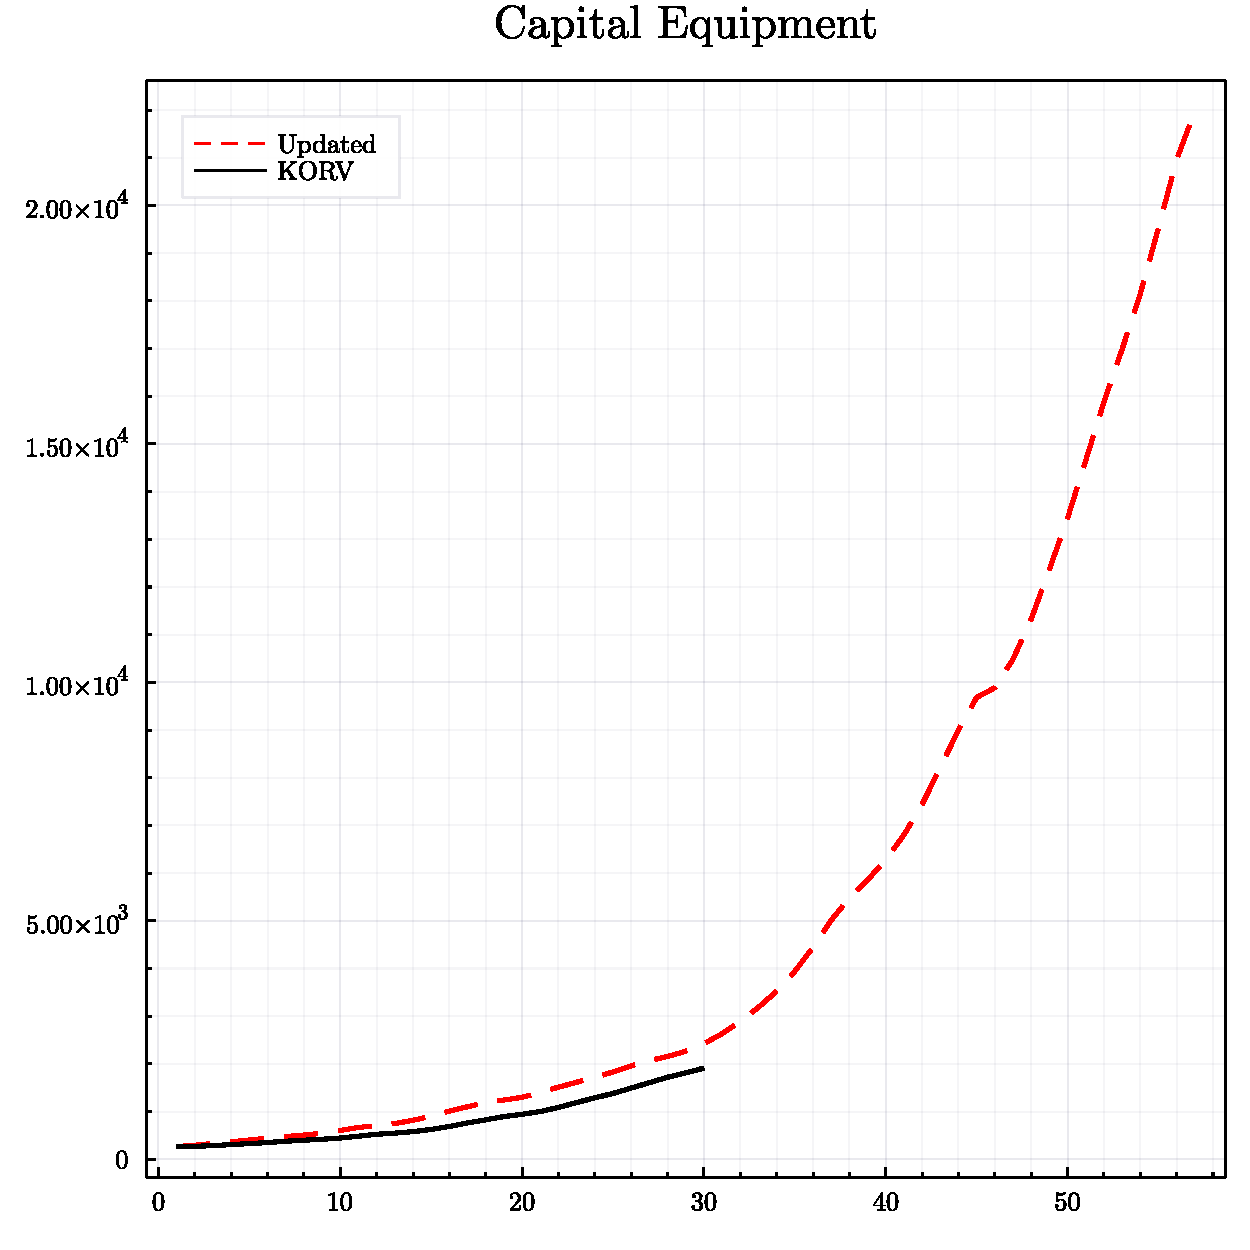
\includegraphics[width=0.3\textwidth]{../images/capital_equipment_doc.pdf}
\hfill
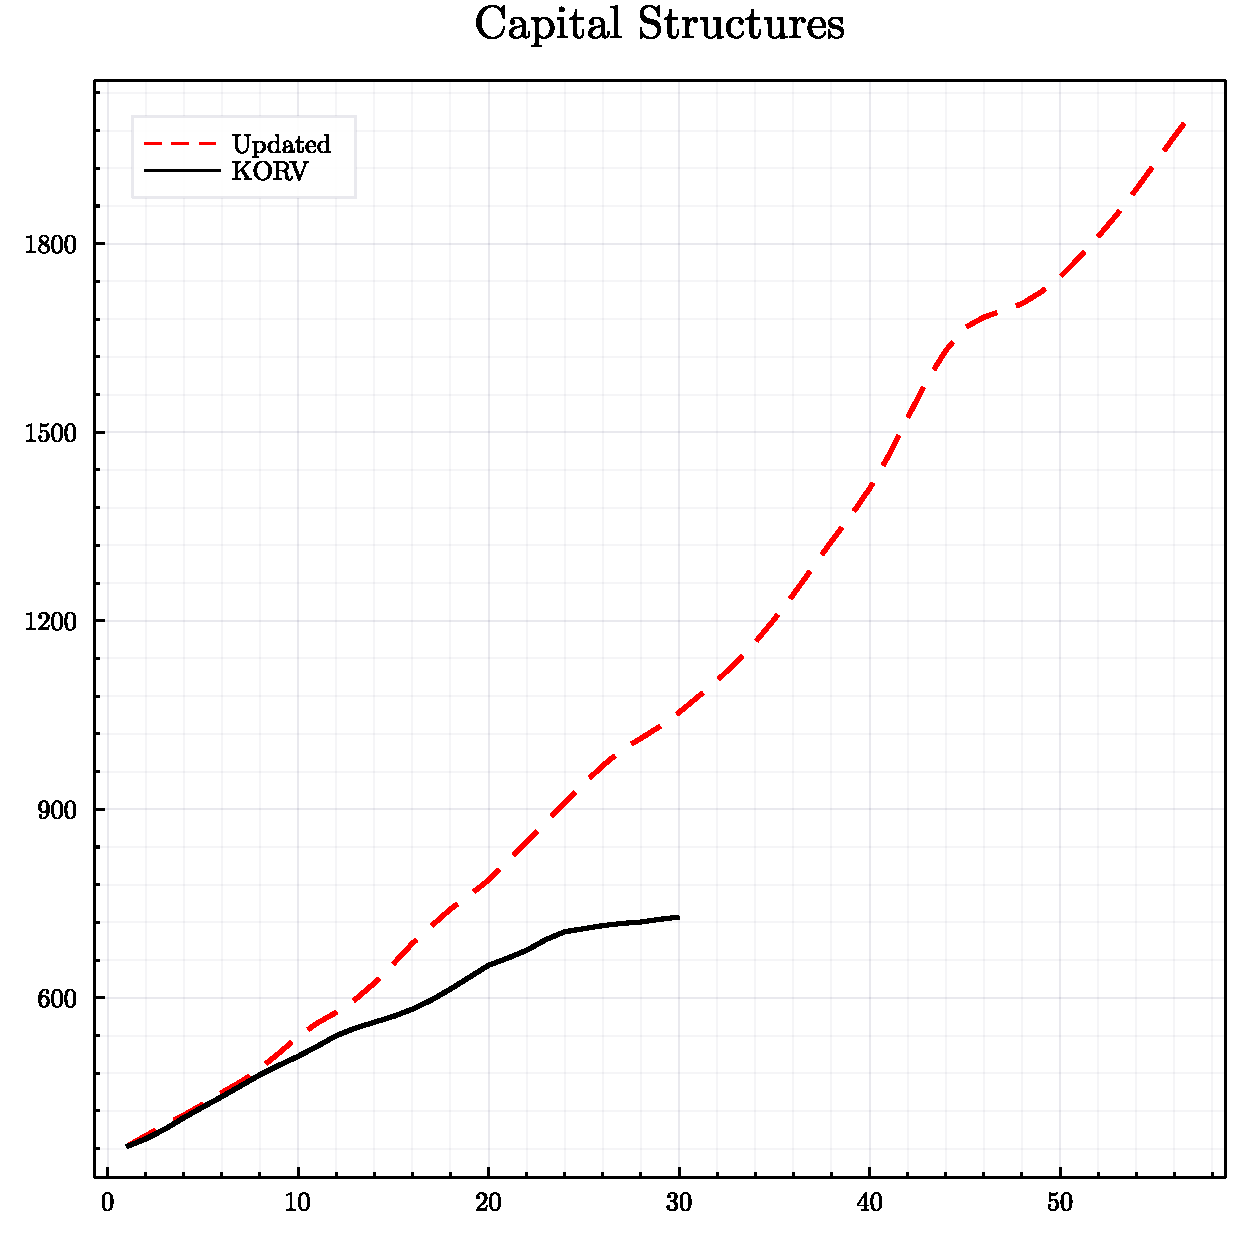
\includegraphics[width=0.3\textwidth]{../images/capital_structures_doc.pdf}
\hfill
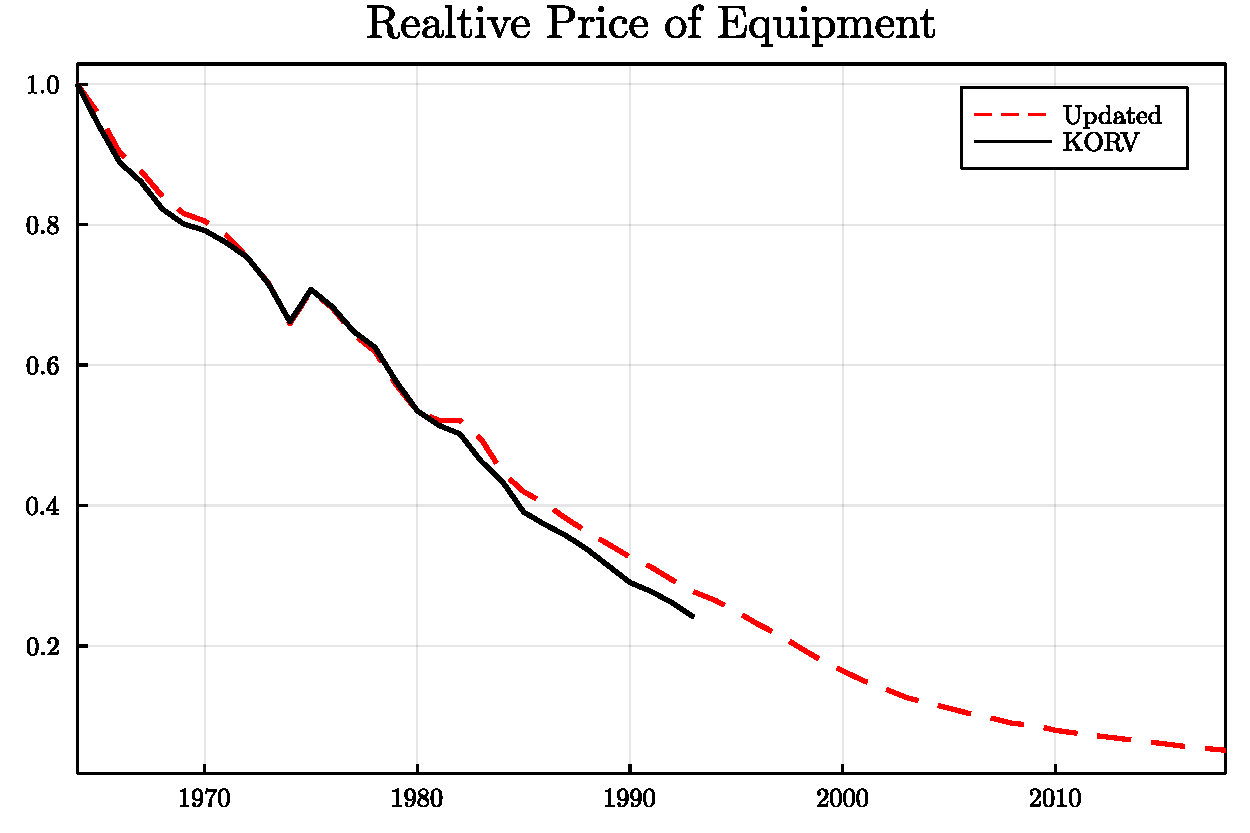
\includegraphics[width=0.3\textwidth]{../images/capital_price_doc.pdf}
\caption{\label{fig:capital_series} Capital Series}
\end{figure}

To obtain capital data at the industry level I used the BEA Fixed Assets dataset to obtain investment and capital consumption series by industry and type, details of which tables were used are included in Appendix \ref{subsec:capital-inputs-labor-share}. Fixed Assets dataset groups industries into 76 groups. To construct a series of the labor share of output by industry, I used the BEA-BLS Integrated Industry-level Production Accounts (KLEMS)\footnote{Available at \url{https://www.bls.gov/productivity/articles-and-research/industry-production-account-capital.xlsx}}. This dataset contains the data underlying the BEA/BLS Integrated Industry-level Production Account for the United States. The data covers 1987-2020. KLEMS data consists of 57 industry groups some of which are aggregations of industries on the BEA dataset. The table 
presents the crosswalk between BEA, KLEMS, and Census industry codes. I used the crosswalk provided by \citep{acemoglu2020unpacking}. A description of the codes is in \textcolor{red}{INSER TABLE AND REFERENCEIT}.

\subsection{Labor Data}\label{sec:labor_data}

Labor input and wages are estimated using the march supplement of the Current Population Survey (CPS), downloaded from IPUMS\footnote{\url{https://cps.ipums.org/cps/index.shtml}}, see \citet{flood2015integrated}. Flowing \citep{krusell2000capital} and \citep{ohanian2021revisiting} I include all observations excluding agents: younger than $16$ or older than $70$, unpaid family workers, those working in the military, those who report working less than $40$ weeks a year and/or $35$ hours a week, individuals with allocated income, those with hourly wages below half of the minimum federal wage rate, those did not report their education level and self-employed workers. Appendix~\ref{subsec:labor-inputs-wage-rates} describes in detail the cleaning process undertaken to obtain the labor input and wage series. Figure~\ref{fig:labor_series} displays the labor input and wage series for the $1963$ - $2018$ period compared with the original data.



\begin{figure}
 \centering
 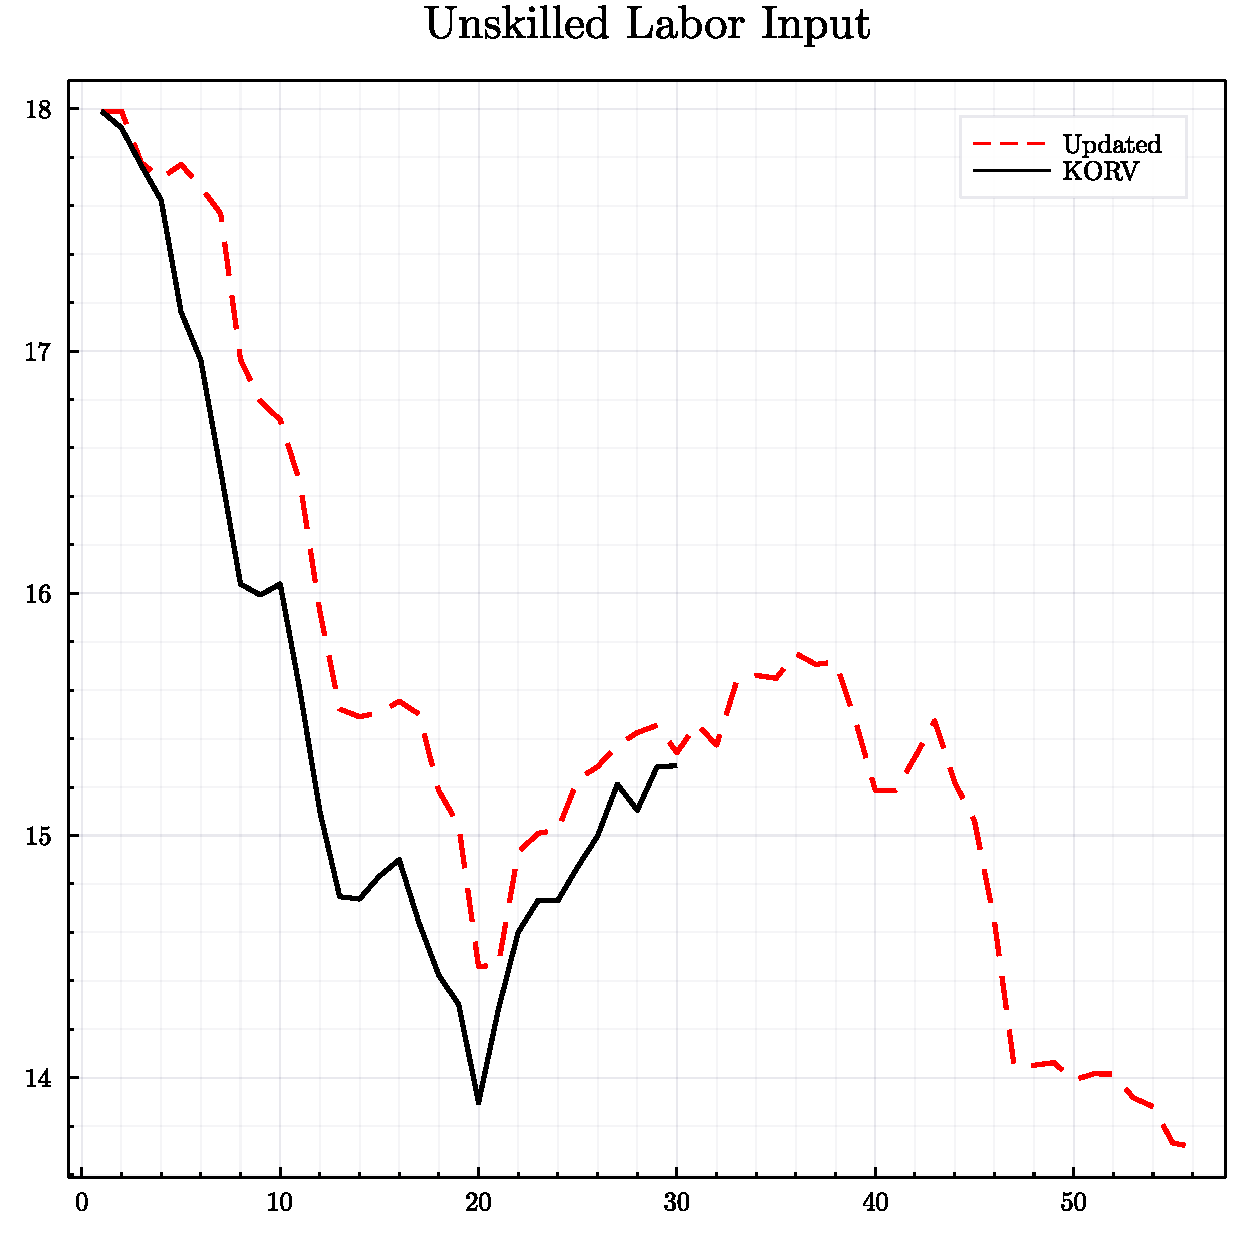
\includegraphics[width=0.45\textwidth]{../images/labor_input_unskilled_doc.pdf}
 \hspace*{0.05\textwidth}
 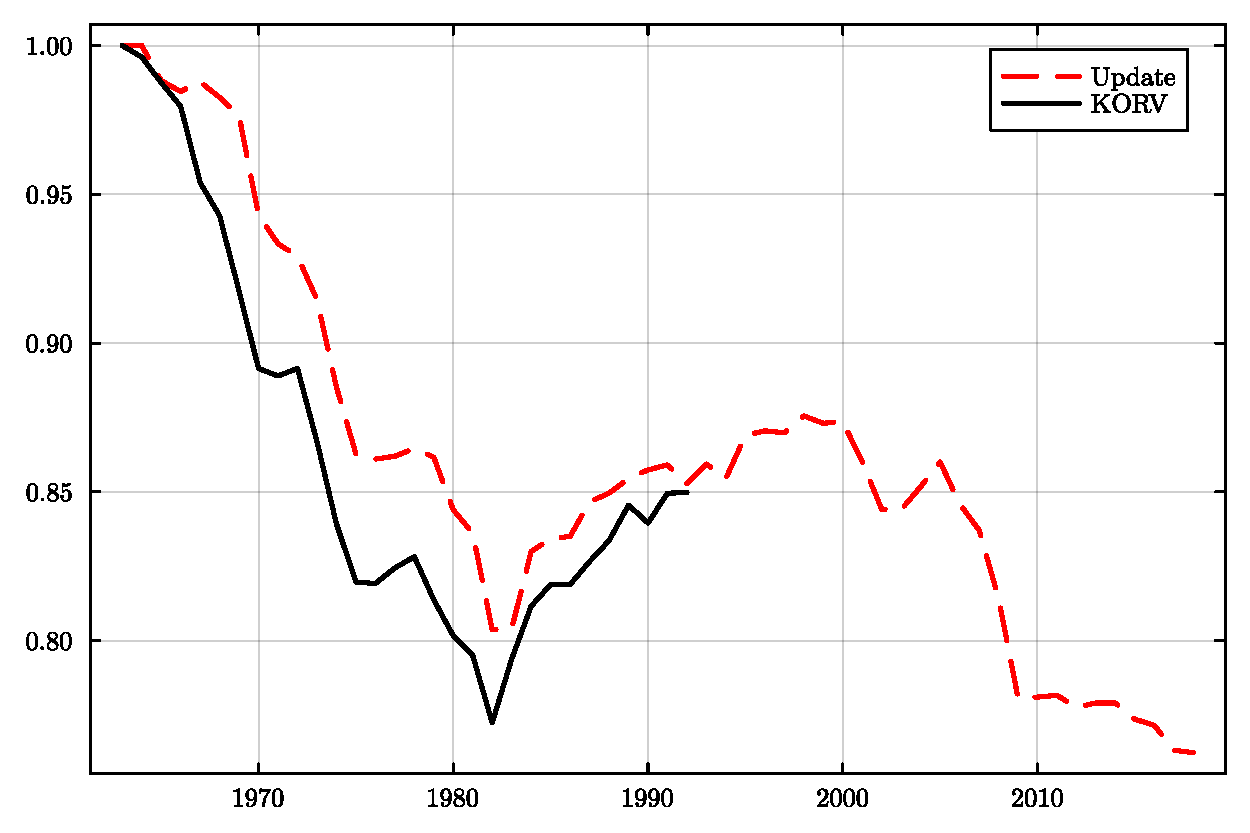
\includegraphics[width=0.45\textwidth]{../images/labor_input_skilled_doc.pdf}
 \vfill
 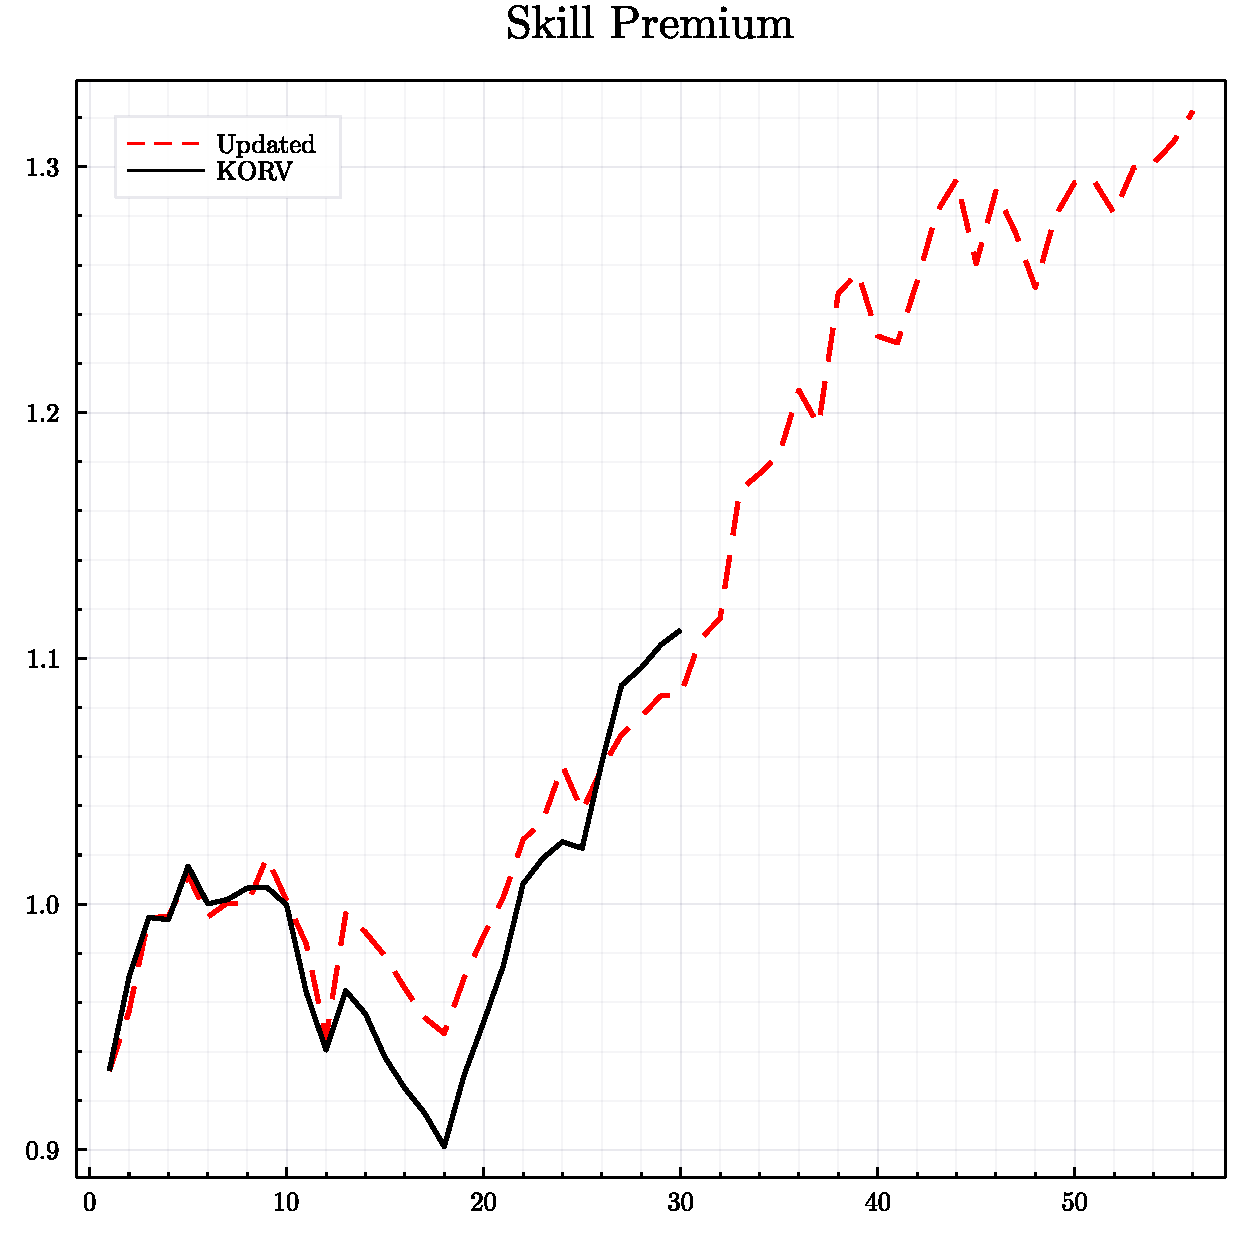
\includegraphics[width=0.45\textwidth]{../images/sp_doc.pdf}
 \hspace*{0.05\textwidth}
 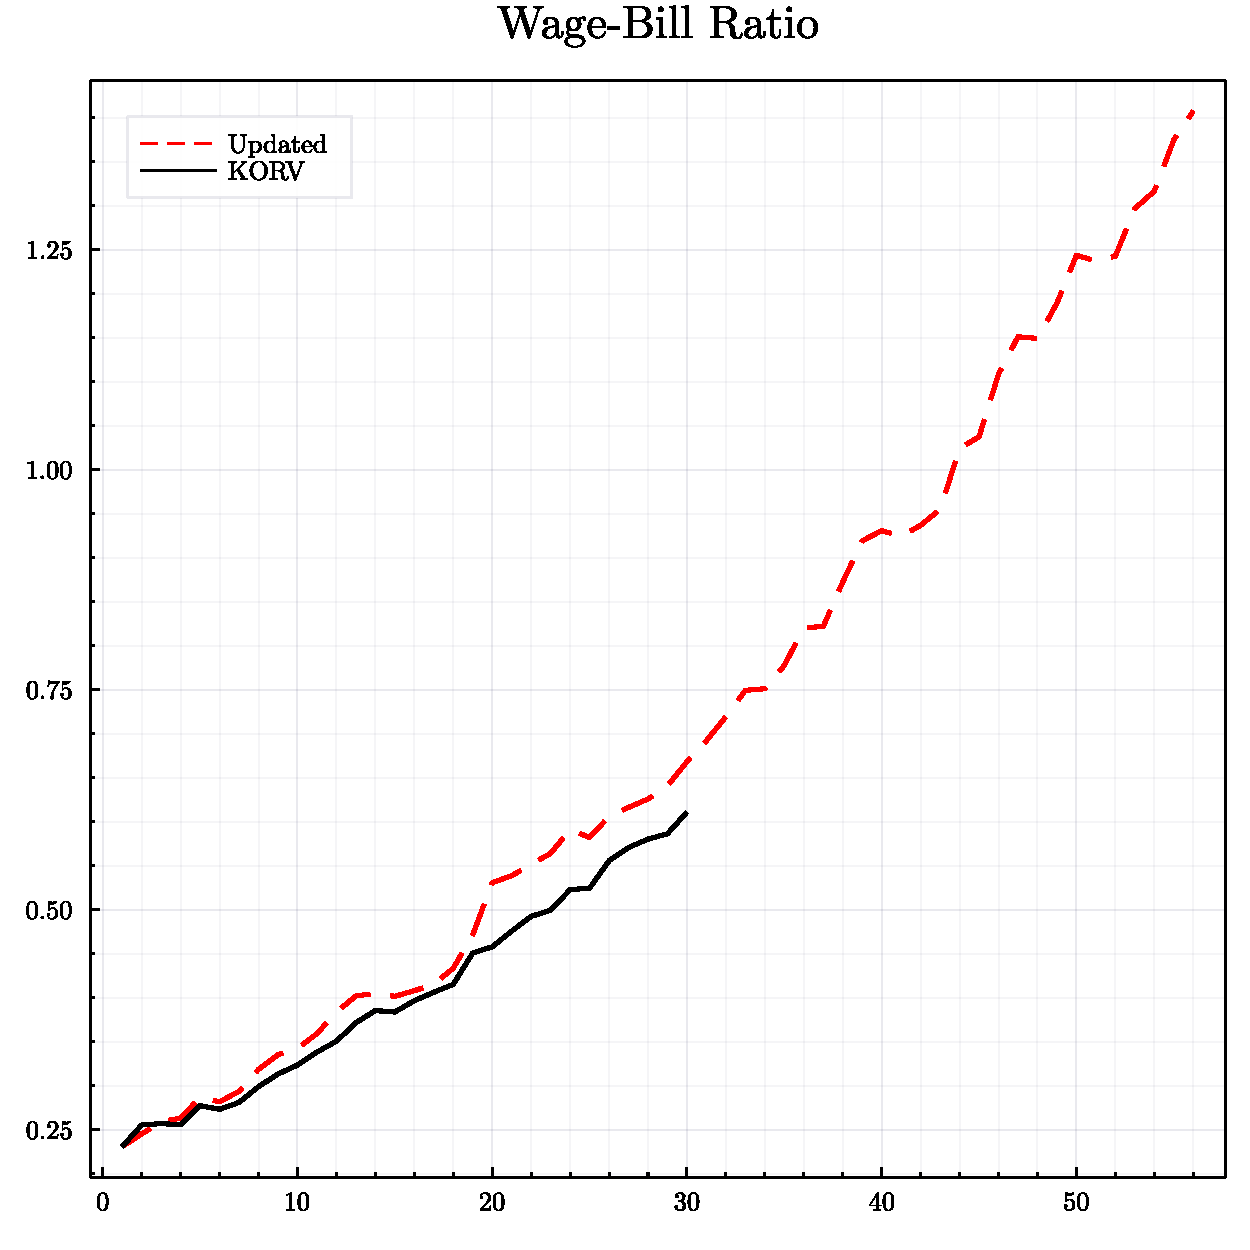
\includegraphics[width=0.45\textwidth]{../images/wbr_doc.pdf}
 \caption{\label{fig:labor_series} Labor Series}
\end{figure}


I used the crosswalk in Table \textcolor{red}{INSER TABLE AND REFERENCEIT} to group Census code groups for each industry and subdivided the original CPS data. I then repeated the process described in Appendix~\ref{subsec:labor-inputs-wage-rates} to obtain labor input and wage series for each industry.


\subsection{Labor Income Shares}\label{sec:labor_share_income}
To construct labor share series at the economy level I follow \citet{krusell2000capital}, \citet{castex2022decline} and \citet{ohanian2021revisiting} in following the \citet*{cooley1995frontiers}. I first generate a series containing capital income $(CI)$ consisting of the sum of 
\begin{enumerate}[(i)]
 \item net interest and miscellaneous payments, domestic industries,
 \item corporate profits,
 \item consumption of fixed capital.
\end{enumerate}
Capital share is defined as the ratio between $CI$ and gross domestic income (net of proprietors' income) $Y - PI$. Labor share is then calculated as 
\begin{equation*}
 LI = 1 - \frac{CI}{Y - PI}
\end{equation*}

To construct labor share series at the industry level, I used the BEA-BLS Integrated Industry-level Production Accounts (KLEMS). KLEMS dataset contains information on the compensation of employees (with and without a college degree) and the value added by industry, I then follow \citep{karabarbounis2014global} and define the labor share as the ratio between the total compensation of employees and the total value added by industry.

\begin{figure}[H]
\centering
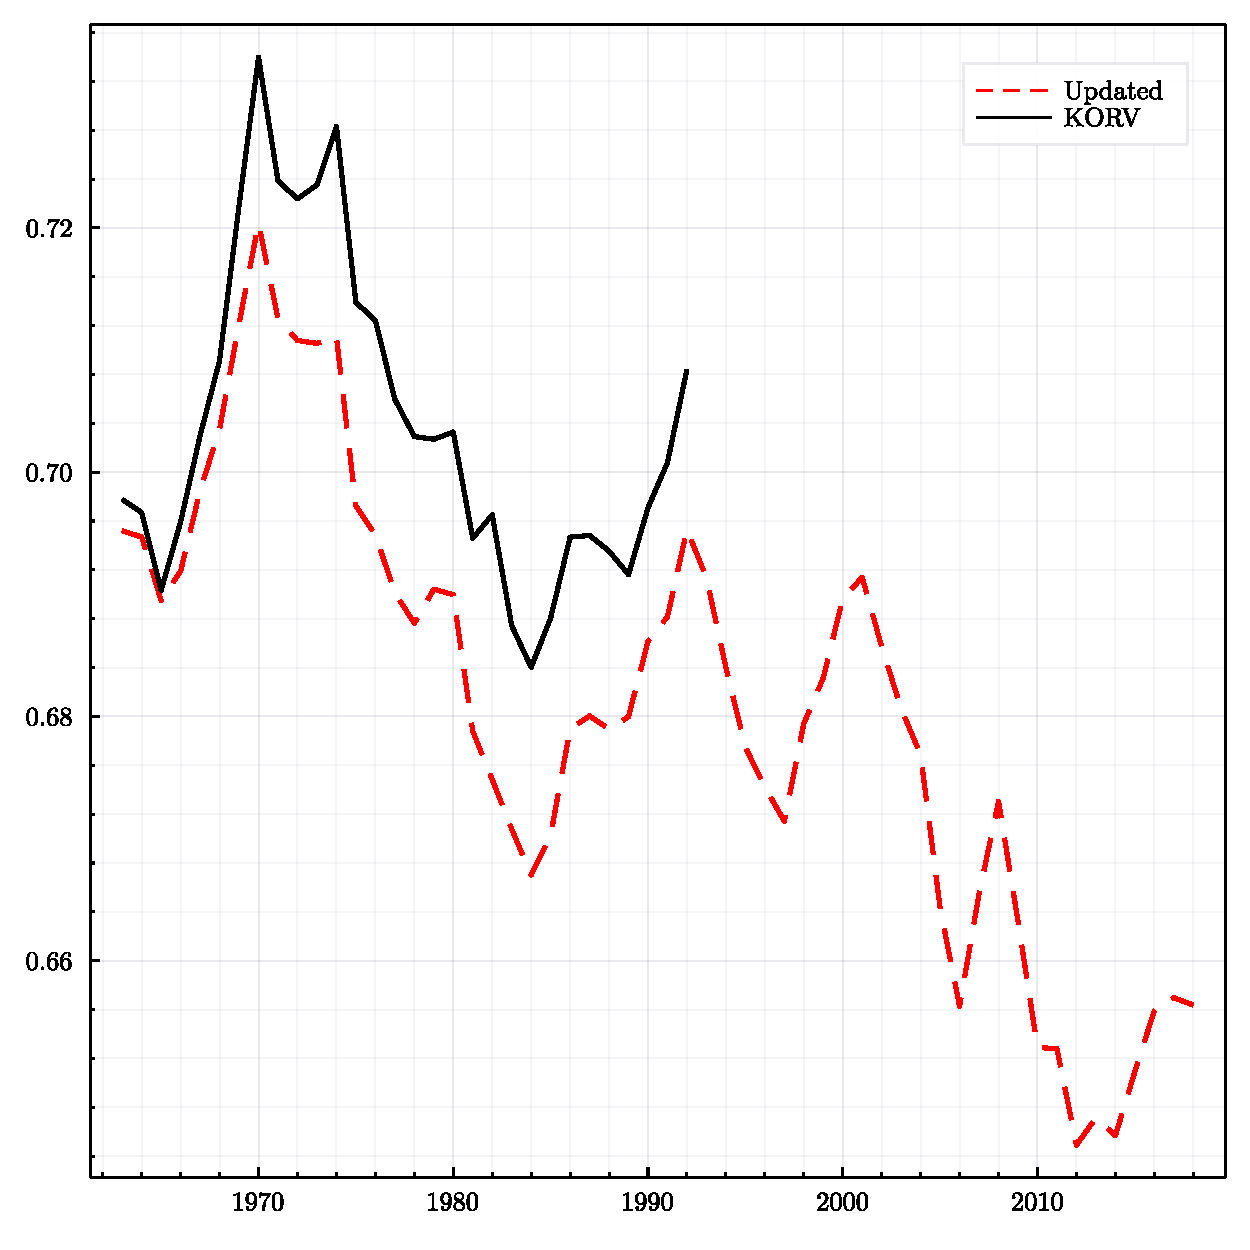
\includegraphics[width=0.5\textwidth]{../images/fig:labor_share_updated.pdf}
\caption*{\label{fig:labor_share_updated} Labor Share of Income}
\end{figure}

\subsection{Data Description}

\subsubsection{Industry Trends}

The trend of the labor share in the industry is the same at the national level Figure~\ref*{fig:labor_share_by_industry}

\begin{figure}[H]
 \centering
 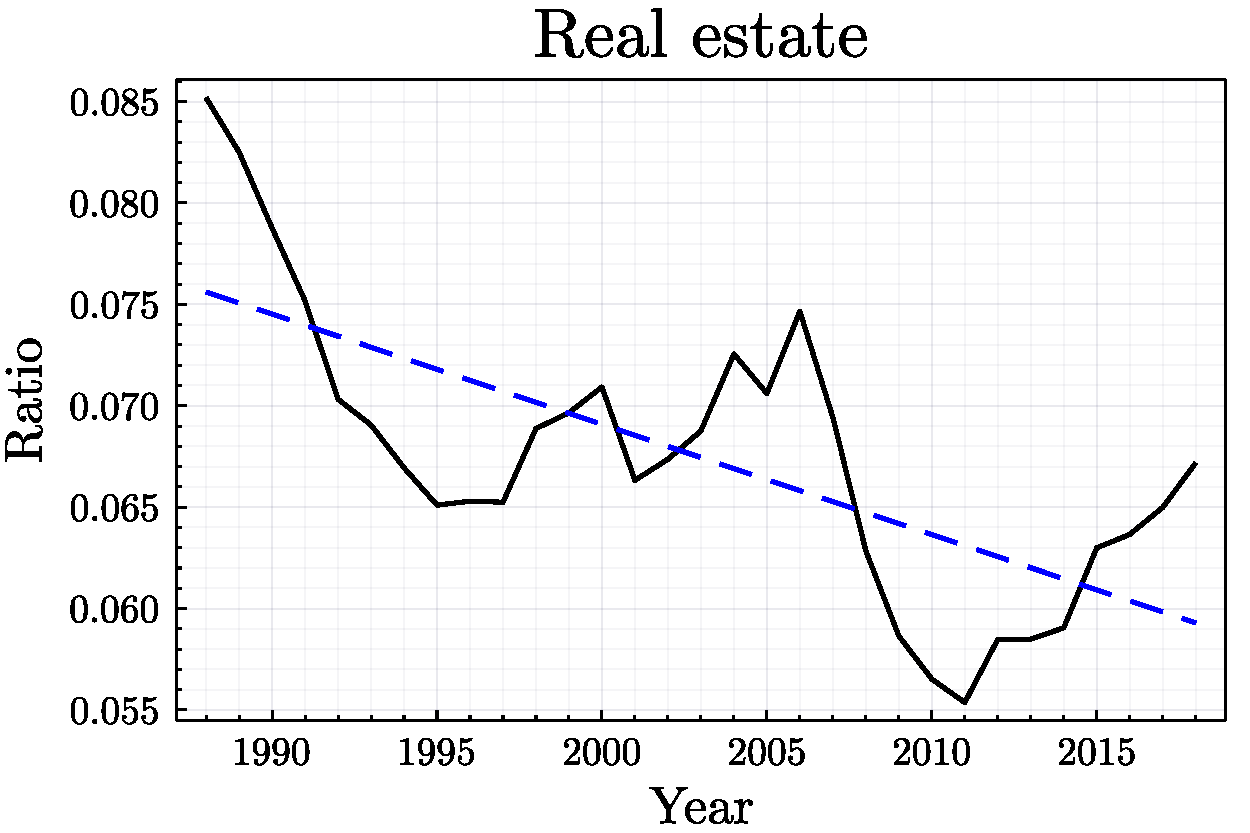
\includegraphics[width=0.45\textwidth]{../images/industries/labor_share/dec531.pdf}
 \hspace*{0.05\textwidth}
 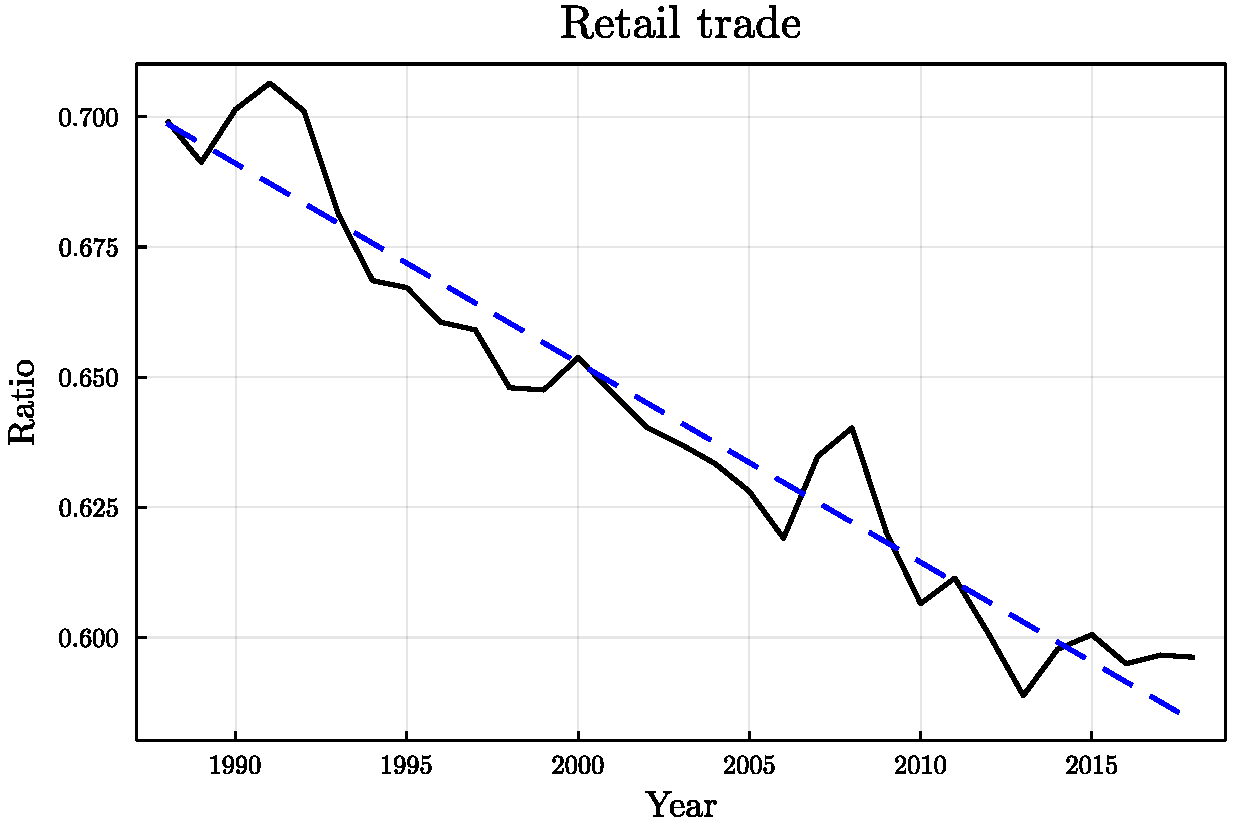
\includegraphics[width=0.45\textwidth]{../images/industries/labor_share/dec44RT.pdf}
 \vfill
 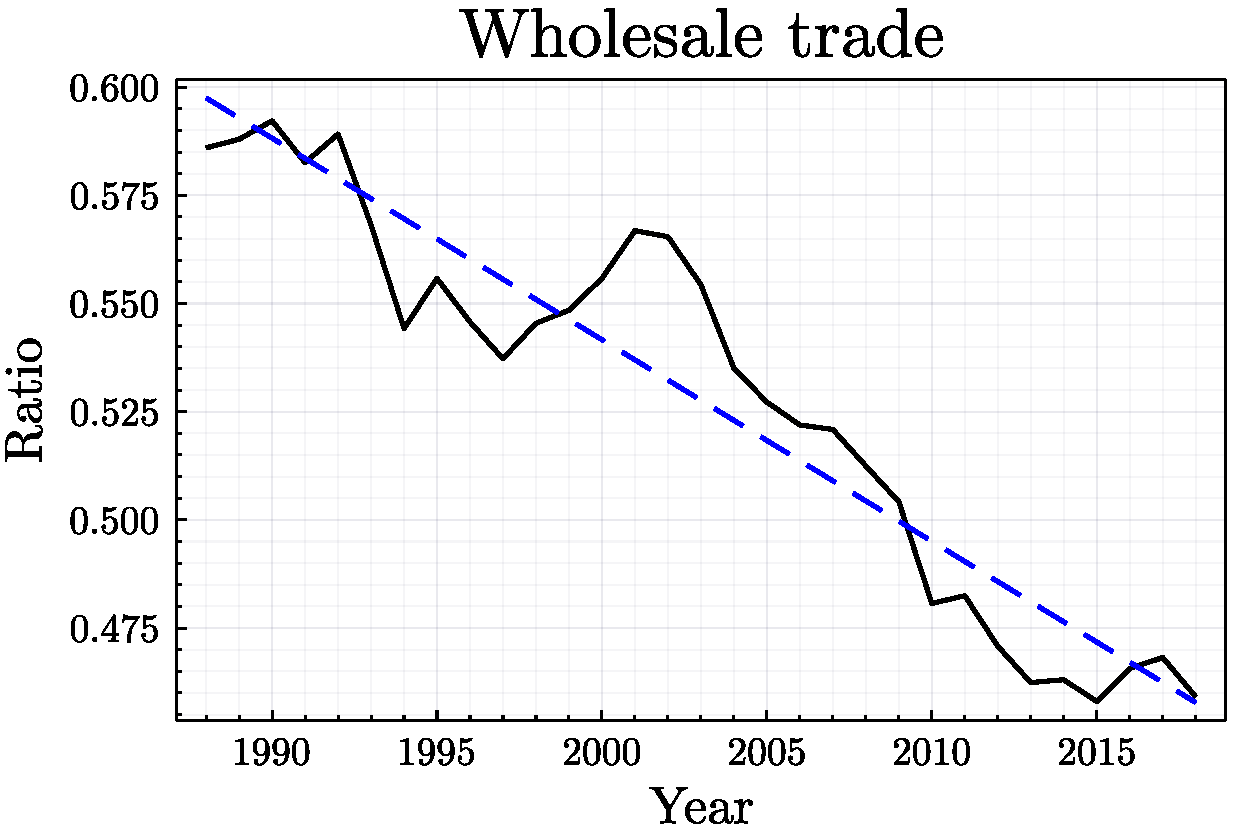
\includegraphics[width=0.45\textwidth]{../images/industries/labor_share/dec42.pdf}
 \hspace*{0.05\textwidth}
 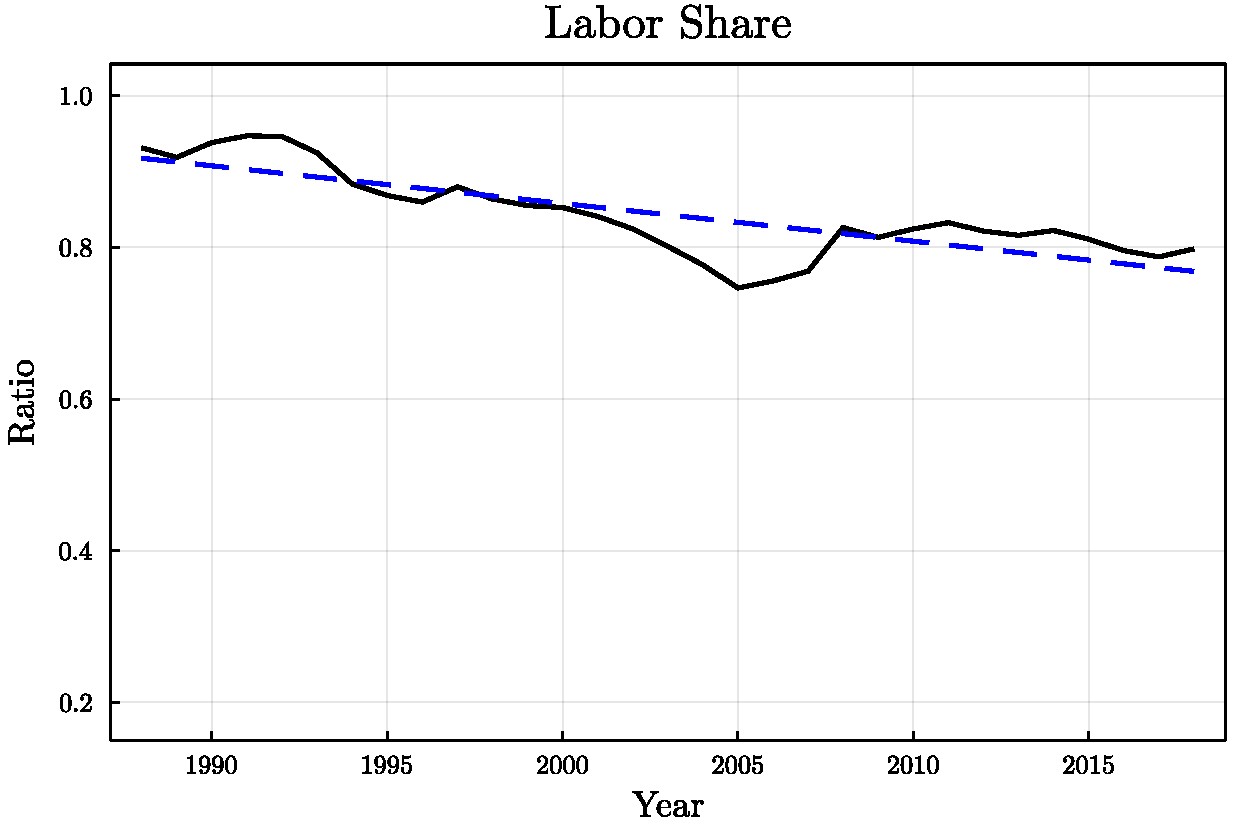
\includegraphics[width=0.45\textwidth]{../images/industries/labor_share/dec23.pdf}
 \caption{\label{fig:labor_share_by_industry} Declining Labor Share four larges industries}
\end{figure}

To justify exploring the skill-biased technical change I want to show that the feature of increasing labor input ratio holds and also the skill premium increasing holds at the industry level.

I calculate the slope of the labor input and get that \textcolor{red}{RESULTS}, I then repeat the process for the skill premium and get the \textcolor{red}{RESULTS}. Figure~\ref*{fig:trends_correlation} shows a scatter plot of slopes. The first thing to note is that for almost all industries (\textcolor{red}{percentage}) there;'s been an increase in both indicators, furthermore the more that labor input ratio increases the more the skill premium increases. 

Figure~\ref{fig:trends_correlation} shows \ldots

\begin{figure}[H]
 \centering
 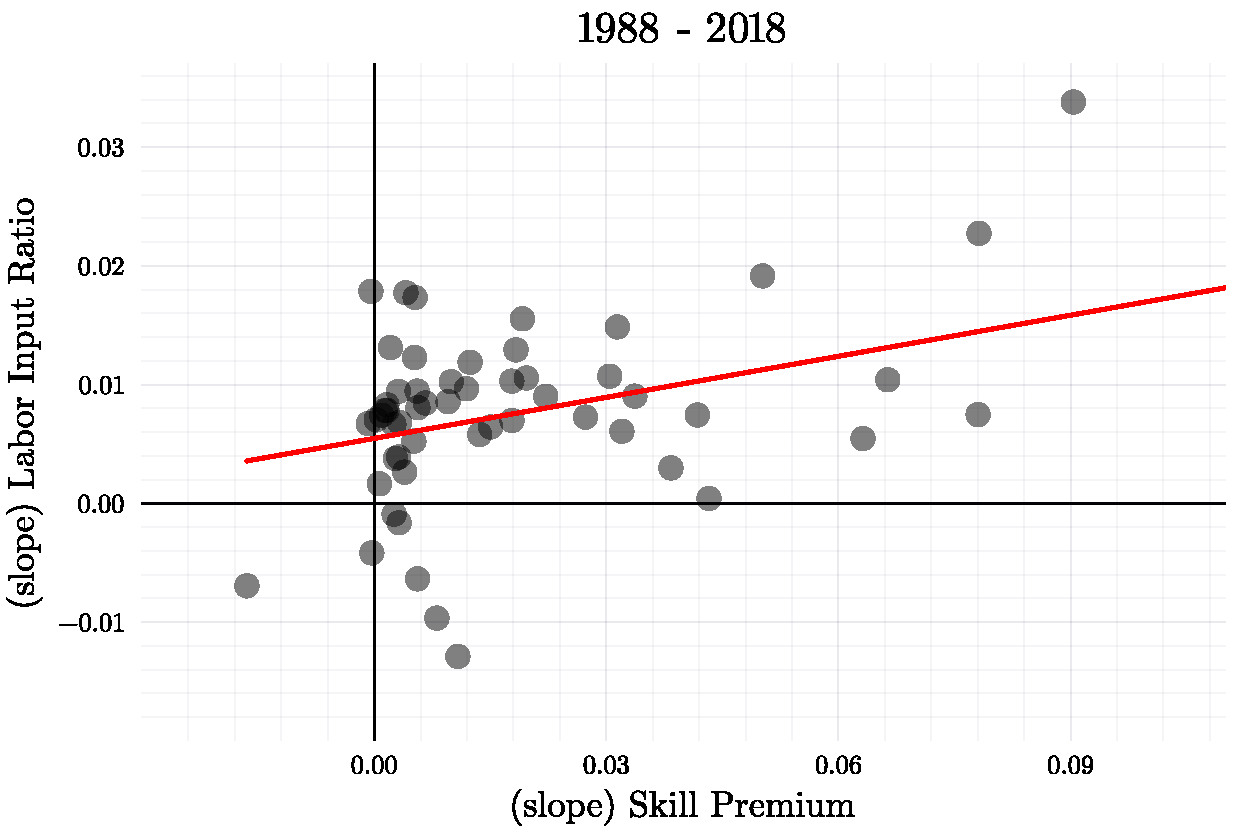
\includegraphics[width=0.85\textwidth]{../images/trend_correlation_doc.pdf}
 \caption{\label{fig:trends_correlation} Correlation between the slopes of the Labor Input Ration and the Skill Premium.}
\end{figure}

\section{Model}\label{sec:model}
This section presents the model which is the same as \citep{krusell2000capital}. There are four inputs for production in this economy: two types of capital, equipment $(k_e)$ and structures $(k_s)$ and two types of labor, skilled $(s)$ and unskilled $(u)$. Inputs are combined through a production function $G(\cdot)$ to produce three final goods: consumption $(c)$, investment in equipment $(i_e)$ and investment in structures $(i_s)$. Assuming a hicks-neutral technological shock $A$, the aggregate production is given by
\begin{equation}\label{eq:production}
 c_t + i_{e_t} + i_{s_t} = Y_t = A_t G(k_{s_t}, k_{e_t}, u_t, s_t)
\end{equation}
Capital evolves following the law of motion in \eqref{eq:capital_law_motion}. The production function is assumed to be Cobb-Douglas in structures and a nested CES in all other inputs:
\begin{equation}\label{eq:production_fun}
 G(k_{s_t}, k_{e_t}, u_t, s_t) = k_{s_t}^\alpha\left( \mu u_t^\sigma + (1-\mu)\left(\lambda k_{s_t}^\rho (1-\lambda)s_t^\rho\right)^\frac{\sigma}{\rho}\right)^\frac{1-\alpha}{\sigma}
\end{equation}
where $\alpha$ is the share of capital structures in output, $\mu$, and $\lambda$ are income shares, $\rho$ and $\sigma$ govern the elasticity of substitution between capital equipment and labor:
\begin{itemize}
 \item $\sigma_s = 1/(1-\rho)$ is the elasticity of substitution between equipment and high-skilled.
 \item $\sigma_u = 1/(1-\sigma)$ is the elasticity of substitution between low-skilled and equipment + high skill labor.
\end{itemize}
Labor input is defined as 
\begin{align*}
    u &= \psi^u_t h^u_t\\
    s &= \psi^s_t h^s_t
\end{align*}
where $\psi^i_t$ is the (unobserved) efficiency of each type of labor and $h^i_t$ is the number of labor hours. 

\subsection{Skill Premium}
The model can be used to analyze the determinants of the skill premium growth, i.e. growth of the ratio of wages of skilled labor to wages of unskilled labor. 

Firms solve the following profit maximization problem 
\begin{equation}\label{eq:profit_max}
 \max_{k_{s_t}, k_{e_t}, u_t, s_t} G(k_{s_t}, k_{e_t}, u_t, s_t) - r_{s_t}k_{s_t} - r_{e_t}k_{e_t} - w_{u_t} h_{u_t} - w_{s_t} h_{s_t}
\end{equation}
$r_{s_t}$ and $r_{e_t}$ are rental rates of capital and $w_{u_t}$ and $w_{s_t}$ are wages of unskilled and skilled workers. Assuming perfect competition, labor is paid it marginal productivity therefore the skill premium at time $t$, ($\omega_t$) is given by
\begin{equation}
 \omega_t = \frac{w_{s_t}}{w_{u_t}} = \frac{G_{h_s}(k_{s_t}, k_{e_t}, u_t, s_t) }{G_{h_u}(k_{s_t}, k_{e_t}, u_t, s_t) }
\end{equation}

this gives the following expression for the skill premium:

\begin{equation}\label{eq:skill_premium}
 \omega_{t}=\frac{(1-\mu)(1-\lambda)}{\mu}\left[\lambda\left(\frac{k_{e_t}}{s_{t}}\right)^{\rho}+(1-\lambda)\right]^{(\sigma-\rho) / \rho}\left(\frac{h_{u_t}}{h_{s_t}}\right)^{1-\sigma}\left(\frac{\psi^s_t}{\psi^u_t}\right)^{\sigma} .
\end{equation}
Since the object of interest is the steady state growth of $\omega_t$\eqref{eq:skill_premium} can be log-linearized to obtain the following expression:
\begin{equation}\label{eq:skill_premium_log_linear}
 \ln \omega_{t} \simeq \lambda \frac{\sigma-\rho}{\rho}\left(\frac{k_{e_t}}{s_{t}}\right)^{\rho}+(1-\sigma) \ln \left(\frac{h_{u_t}}{h_{s_t}}\right)+\sigma \ln \left(\frac{\psi^s_t}{\psi^u_t}\right)
\end{equation}
Which in turn can be written in terms of growth rates:
\begin{equation}\label{eq:skill_premium_growth_rates}
 \begin{aligned}
 g_{\omega t} \simeq &(1-\sigma)\left(g_{h_{u_t}}-g_{h_{s_t}}\right)+\sigma\left(g_{\psi^s_t}-g_{\psi^u_t}\right) \\
 &+(\sigma-\rho) \lambda\left(\frac{k_{e_t}}{s_{t}}\right)^{\rho}\left(g_{k_{e_t}}-g_{h_{s_t}}-g_{\psi^s_t}\right) 
 \end{aligned}
\end{equation}
where $g_x$ denotes the growth rate of variable $x$, details on the derivations are include in Appendix~\ref{sec:derivations}. Equation~\eqref{eq:skill_premium_growth_rates} has the nice property that it is a linear combination of the growth rates of the inputs in the production function, this allows us to decompose the growth rate of the skill premium into three components that are easy to analyze:
\begin{enumerate}[(i)]
 \item $(1-\sigma)(g_{h_{u_t}}-g_{h_{s_t}})$ depends on the growth rate of one type of labor over the other. We assume that both types of labor are substitutes i.e $\sigma_u < 0 \implies (1-\sigma) < 0$ . This means that if skilled labor grows at a faster rate than unskilled labor, will decrease the skill premium.
 \item $\sigma\left(g_{\psi^s_t}-g_{\psi^u_t}\right)$ depends on the growth rate of the productivity of one type of labor over the other. I follow \citep{krusell2000capital} in making the following stochastic assumptions about labor productivity:
 \begin{equation}\label{eq:stochastic_labor_productivity}
 \psi^i_t = \psi^i_0 + \epsilon \qquad \epsilon \sim N(0, \eta_\omega^2) \qquad i\in\{s,u\}
 \end{equation}
 This assumption guarantees that on average $\sigma (g_{\psi^s_t}-g_{\psi^u_t} )$ is constant over time and does not affect the skill premium growth rate. 
 \item $(\sigma-\rho) \lambda\left(\frac{k_{e_t}}{s_{t}}\right)^{\rho}\left(g_{k_{e_t}}-(g_{h_{s_t}}+g_{\psi_{s_t}})\right)$ . This component depends on two factors:
 \begin{enumerate}
 \item The growth rate of equipment relative to the growth rates of skilled labor input. This allows us to characterize the capital-skill complementarity hypothesis as $\sigma > \rho$, if equipment capital grows faster than skilled labor, the skill-premium will increase.
 \item The ratio of capital equipment to efficiency units of skilled labor input (given our assumptions amounts to the growth rate of skilled labor input), this effect will get larger (smaller) over time if $\rho > 0\:$ ($\rho < 0$). 
 \end{enumerate}
\end{enumerate}

\section{Estimation}
I follow the same methodology as \citep{krusell2000capital} to estimate the model parameters. To simplify notation from now on I will refer to the unobservable labor efficiencies as, $\psi_t = \{\psi^u_t, \psi^s_t\}$, the inputs of the production function as $X_t = \{ k_{s_t} , k_{e_t}, h_{s_t}, h_{u_t}\}$ and the set of parameters to be estimated as $\Phi = \{\alpha, \sigma, \rho, \mu, \lambda, \psi^u_0, \psi^s_0, \eta_\omega \}$. 

Firms decide investment in structures based on expectations about future prices $q_{t+1}$. This is captured using a \textit{"no arbitrage"} condition, firms equate marginal returns on investment on both types of capital. On the one hand marginal return on investment in capital structures is given by given by the sum of the marginal product of structures in $t+1$, $A_{t+1} G_{k_s}(X_{t+1}, \psi_{t+1} \mid \Phi )$ and undepreciated structures on $(1-\delta_s)$. On the other hand marginal return on investment in equipment is given by the sum of the marginal product of equipment in next period, $q_t A_{t+1} G_{k_s}(X_{t+1}, \psi_{t+1} \mid \Phi )$ and depreciated structures $\mathbb{E}(q_t/q_{t+1})(1-\delta_e)$ the term $\mathbb{E}(q_t/q_{t+1})$, as in \citep{krusell2000capital} I make the simplifying assumption of 
$(1-\delta_e)\mathbb{E}(q_t/q_{t+1}) =(1-\delta_e)(q_t/q_{t+1}) + \nu_t$ where $\nu_t$ is normally distributed with mean zero and variance $\eta_\nu^2$ this parameter is calibrated using data on $q_t$.\footnote{Since I use the same series of relative prices as KORV I take their calibration of $\eta_\nu = 0.02$}. Putting everything together we have the following equation:
\begin{equation}\label{eq:no_arbitrage}
 A_{t+1} G_{k_s}(X_{t+1}, \psi_{t+1} \mid \Phi ) = q_t A_{t+1} G_{k_s}(X_{t+1}, \psi_{t+1} \mid \Phi ) + (1-\delta_e)\left(\frac{q_t}{q_{t+1}}\right) + \nu_t
\end{equation}

The other two structural equations used to estimate the model compare the labor share observed in the data to labor share predicted by the model $lsh(X_{t+1}, \psi_{t+1} \mid \Phi )$ and the wage-bill ratio observed in the data to wage-bill ratio predicted by the model $wbr(X_{t+1}, \psi_{t+1} \mid \Phi )$:
\begin{align}
 \frac{w_{s_t}h_{s_t} + w_{u_t}h_{u_t} }{Y_t} &= lsh(X_{t}, \psi_{t} \mid \Phi ) \label{eq:labor_share}\\
 \frac{w_{s_t}h_{s_t}}{w_{u_t}h_{u_t}} &= wbr(X_{t}, \psi_{t} \mid \Phi ) \label{eq:wage_bill_ratio}
\end{align}

Since the parameters $\mu, \lambda, \psi^u_0, \psi^s_0$ act as scaling parameters, to estimate the model one must be fixed, I follow \citep{krusell2000capital} in fixing $\psi^s_0$, the initial value of the productivity of skilled labor. When replicating their result on an extended sample I choose to fix $\psi^u_0 = 6$ as in the original, but choose different variants when estimating each industry to improve fitness. Finally, the parameter $\eta_\omega$ is chosen to minimize the distance between the skill premium in the data and the skill premium predicted by the model.

The estimation process is a simulated two-stage pseudo-maximum likelihood estimation (SPMLE) developed by \citep{white1996estimation}. Is reasonable that the choice of labor is influenced by the shocks in labor productivity, therefore skilled and unskilled labor is treated as endogenous. 

To allow for the possible dependence of hours worked on shocks, we use the two-stage SPML developed by, which is similar in spirit to two-stage least squares. We treat skilled and unskilled labor input as endogenous. To deal with the endogeneity, labor input is projected onto a constant, current, and lagged stock of capital equipment and structures, the lagged relative price of equipment, and a trend. The model is estimated using the instrumented labor input series, the series of capital, and prices as the inputs of the model.

The the next stage we proceed as follows: taking the variance $\eta_\omega$ as given, for each date $t$ generate $S$ realizations the stochastic components of the model $\quad \varphi_t$ use those as inputs to generate $S$ realization of the structural equations \eqref{eq:no_arbitrage}, \eqref{eq:labor_share} and \eqref{eq:wage_bill_ratio}, to simplify notation I refer to each of those values as $\tilde{Z}^{i}_t(X_{t}, \psi_{t} \mid \Phi)$, (note that this is a vector of three values, one for each of the equations). Using the simulated data we obtain the first and second moments of the model: 
\begin{equation}\label{eq:first_moment}
 m(X_{t}, \psi_{t} \mid \Phi) = \frac{1}{S}\sum_{i=1}^S \tilde{Z}^{i}_t(X_{t}, \psi_{t} \mid \Phi)
\end{equation}
and
\begin{equation}\label{eq:second_moment}
 V(X_{t}, \psi_{t} \mid \Phi) = \frac{1}{S-1}\sum_{i=1}^S \left( \tilde{Z}^{i}_t(X_{t}, \psi_{t} \mid \Phi) - m(X_{t}, \psi_{t} \mid \Phi) \right) \left( \tilde{Z}^{i}_t(X_{t}, \psi_{t} \mid \Phi) - m(X_{t}, \psi_{t} \mid \Phi) \right)'
\end{equation}
Finally, we minimize the same objective function as \citep{krusell2000capital}:
\begin{equation}\label{eq:objective_funct_estimation}
 \begin{aligned}
 \ell\left(Z^{T} ; X_{t}, \psi_{t} \mid \Phi\right)=&-\frac{1}{2 T} \sum_{t=1}^{T}\left\{\left[Z_{t}-m_{S}\left(\tilde{X}_{t} ; \phi\right)\right]^{\prime}\left(V_{S}\left(\tilde{X}_{t} ; \phi\right)\right)^{-1}\left[Z_{t}-m_{S}\left(\tilde{X}_{t} ; \phi\right)\right]\right.\\
 &\left.-\log \operatorname{det}\left(V_{S}\left(\tilde{X}_{t} ; \phi\right)\right)\right\}
 \end{aligned} 
\end{equation}
where $Z_{t}$ is the vector of model counterparts of $\tilde{Z}^{i}_t(X_{t}, \psi_{t} \mid \Phi)$.
\section{Results}\label{sec:results}
This section presents the results of the estimation process. I first show the result of the replication of KORV for different periods and then summarize the results of estimating the model for each industry.
\subsection{KORV Replication}\label{sec:results_original}
Table~\ref{tab:estimation_korv} compares the results obtained by \citep{krusell2000capital} to this replication using their 
original data ($1963$ - $1992$) \footnote{Available at Gianluca Violante's website: \url{http://violante.mycpanel.princeton.edu/Journals/Data_KORV.txt}}. I present also the estimation on the extended sample ($1963$ - $2018$) and on the subset of the extended sample for which there is coverage at the industry level ($1988$ - $2018$). 

\begin{table}[h]
\begin{center}
 \begin{tabular}{rrrrr}
  \hline\hline
   & \textbf{KORV Estimation} & \textbf{Replication} & \textbf{Updated Data} & \textbf{Updated Data} \\
   & \texttt{$1963$ - $1992$} & \texttt{$1963$ - $1992$} & \texttt{$1963$ - $2018$} & \texttt{$1988$ - $2018$} \\\hline
  $\alpha$ & 0.117 & 0.113 & 0.118 & 0.08 \\
  $\sigma$ & 0.401 & 0.464 & 0.503 & 0.313 \\
  $\rho$ & -0.495 & -0.56 & -0.343 & -0.154 \\
  $\eta_\omega$ & 0.043 & 0.043 & 0.083 & 0.043 \\\hline\hline
\end{tabular}

 \caption{\label{tab:estimation_korv} Parameter estimates KORV model.}
\end{center}
\end{table}

Table~\ref{tab:estimation_elasticities_korv} compares elasticities of substitution implied by the different parameter estimates obtained.

\begin{table}[h]
 \begin{center}
 \begin{tabular}{rrrrr}
  \hline\hline
   & \textbf{KORV Estimation} & \textbf{Replication} & \textbf{Updated Data} & \textbf{Updated Data} \\
   & \texttt{$1963$ - $1992$} & \texttt{$1963$ - $1992$} & \texttt{$1963$ - $2018$} & \texttt{$1988$ - $2018$} \\\hline
  $\sigma_s$ & 0.668896 & 0.641107 & 0.744831 & 0.857268 \\
  $\sigma_u$ & 1.66945 & 1.86506 & 2.01136 & 1.8599 \\\hline\hline
\end{tabular}

 \caption{\label{tab:estimation_elasticities_korv} Implied Elastities of Substitution}
 \end{center}
 \end{table}

Figures~\ref{fig:korv_estimation},~\ref{fig:korv_estimation_extended} and~\ref{fig:korv_estimation_extended_industry} show the fit of the estimation process for three samples decribed. 


\begin{figure}[H]
 \centering
 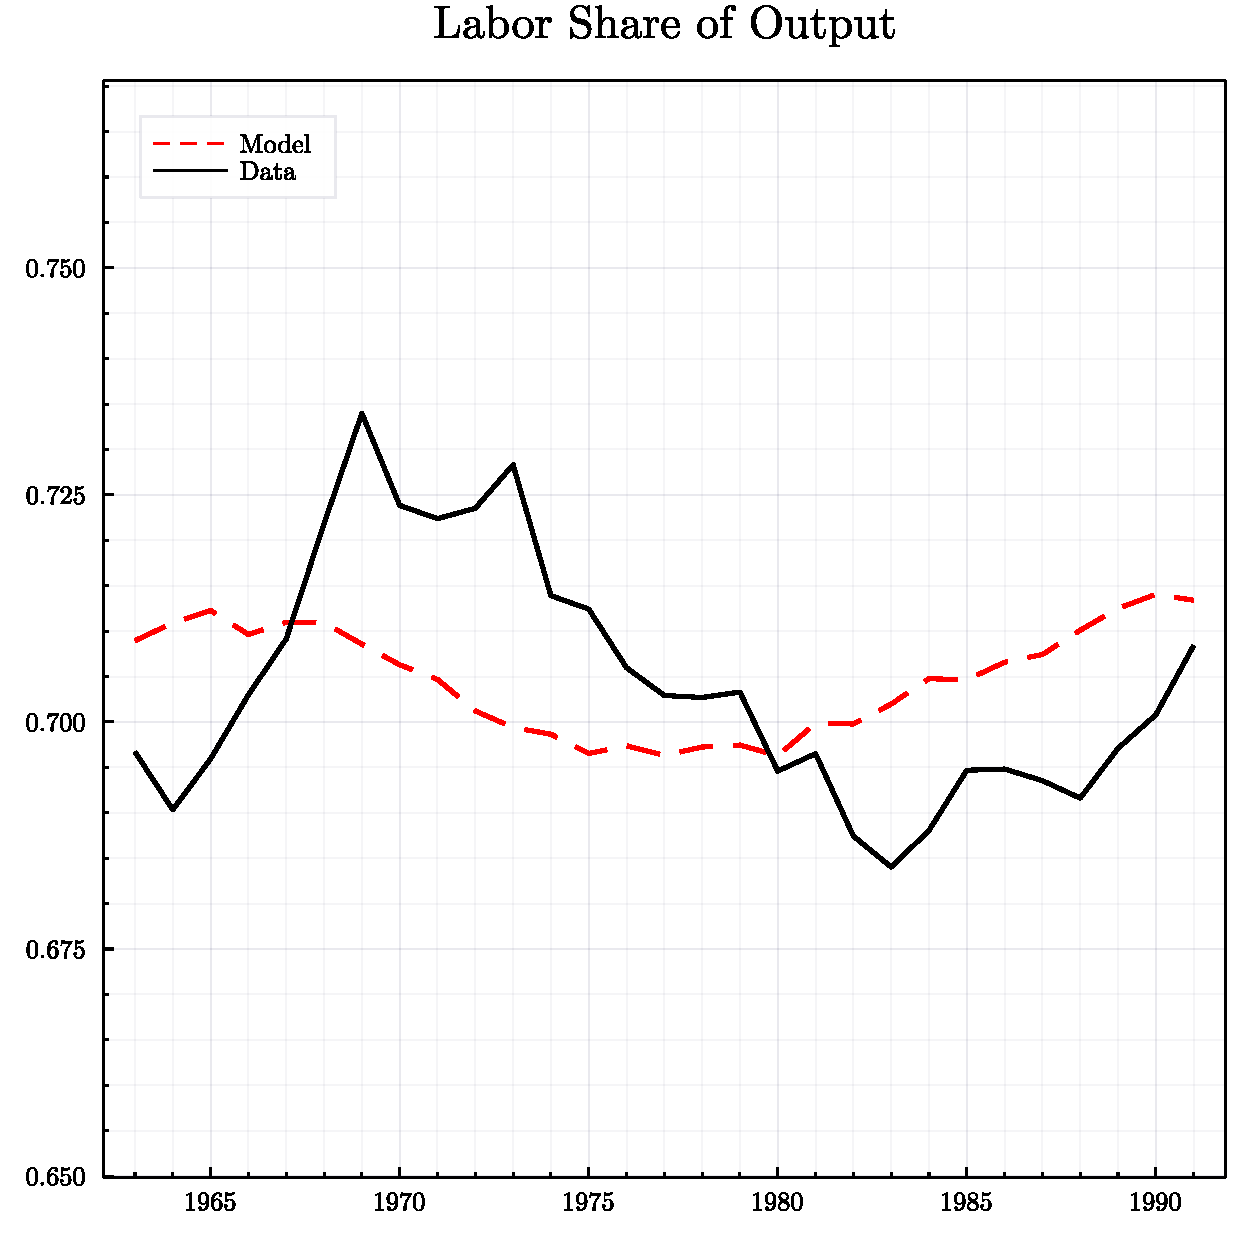
\includegraphics[width=0.3\textwidth]{../images/fig:korv_estimation_ls_doc.pdf}
 \hfill
 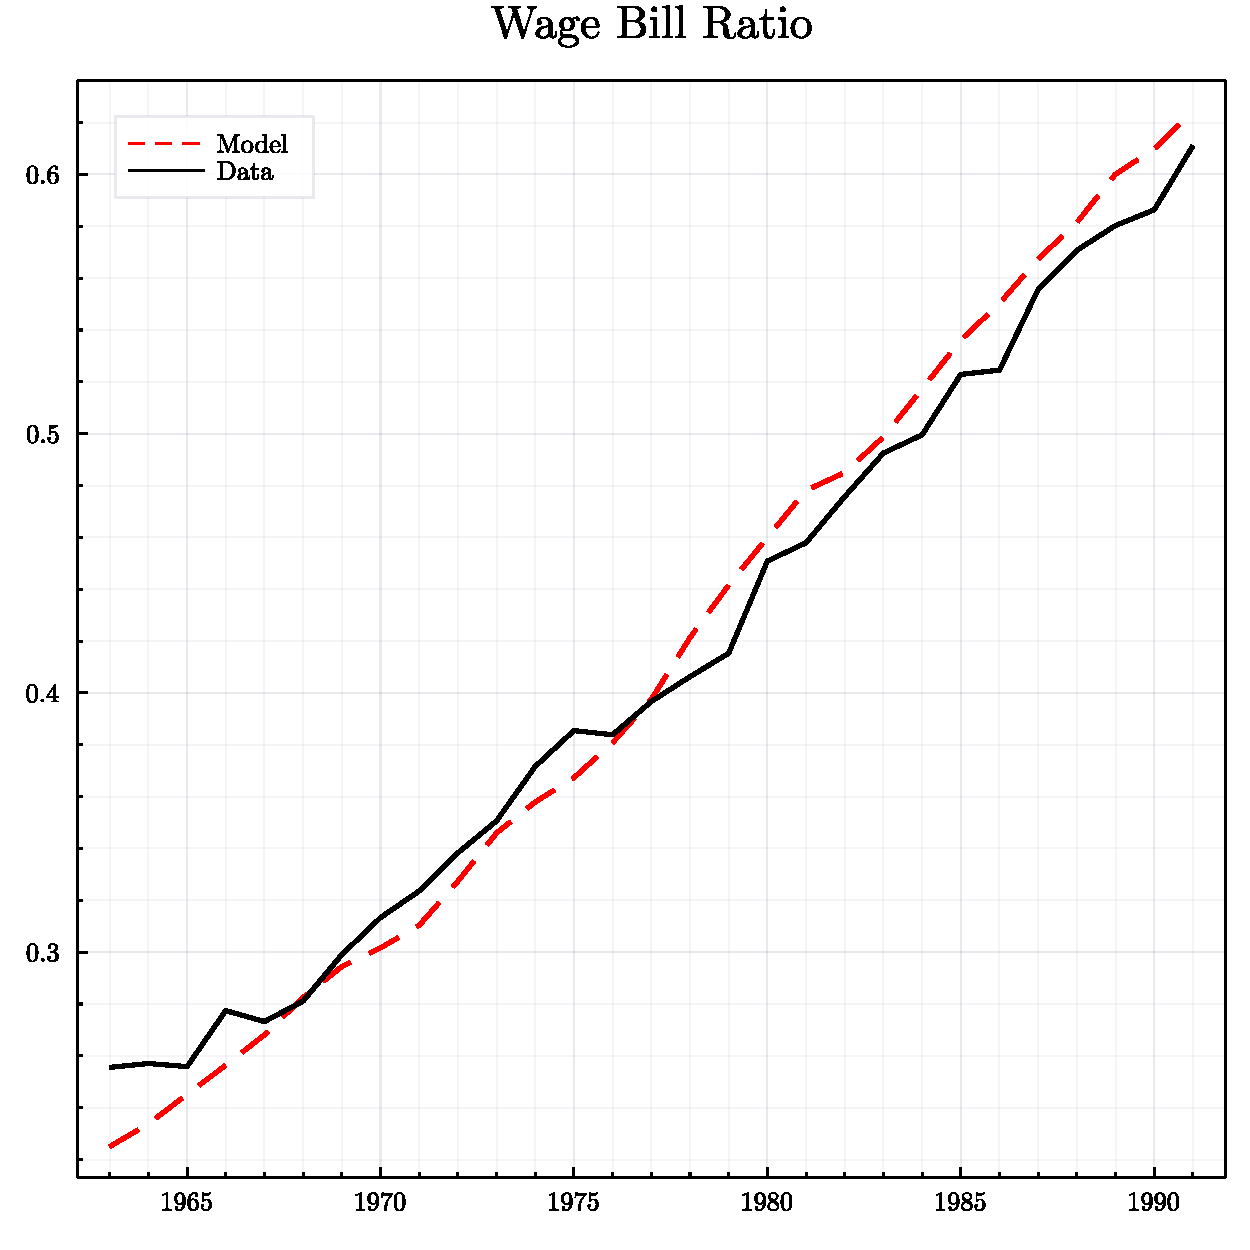
\includegraphics[width=0.3\textwidth]{../images/fig:korv_estimation_wbr_doc.pdf}
 \hfill
 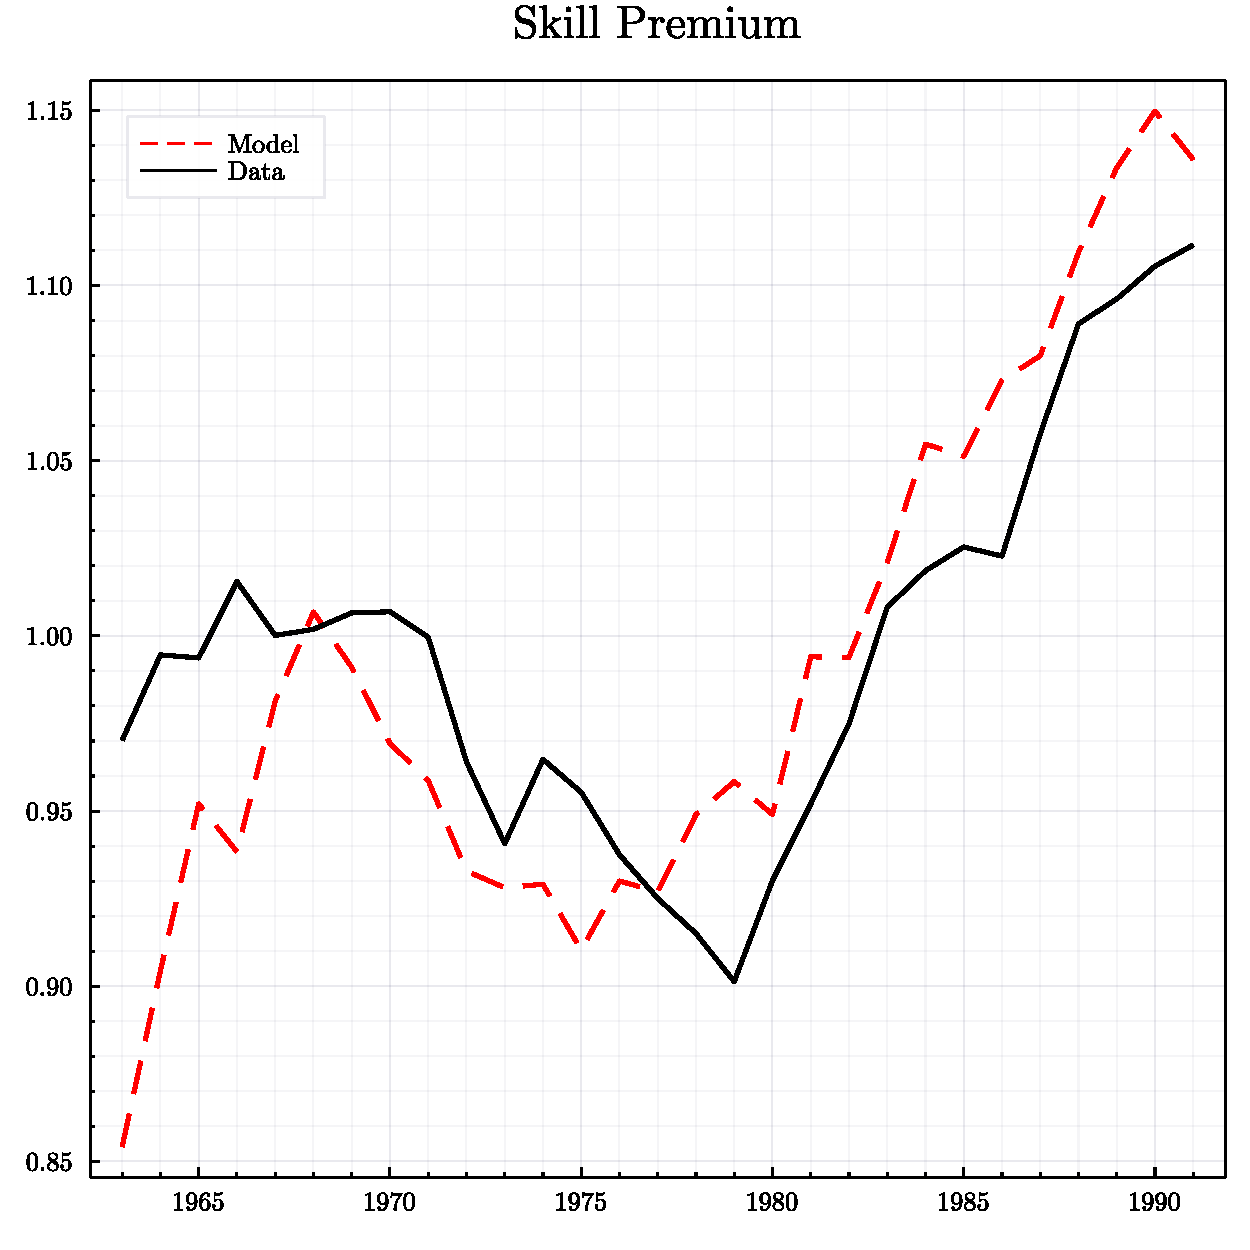
\includegraphics[width=0.3\textwidth]{../images/fig:korv_estimation_sp_doc.pdf}
 \caption{\label{fig:korv_estimation} The model Fit for the $1963$ - $1992$ period with KORV Data.}
\end{figure}
\begin{figure}[H]
 \centering
 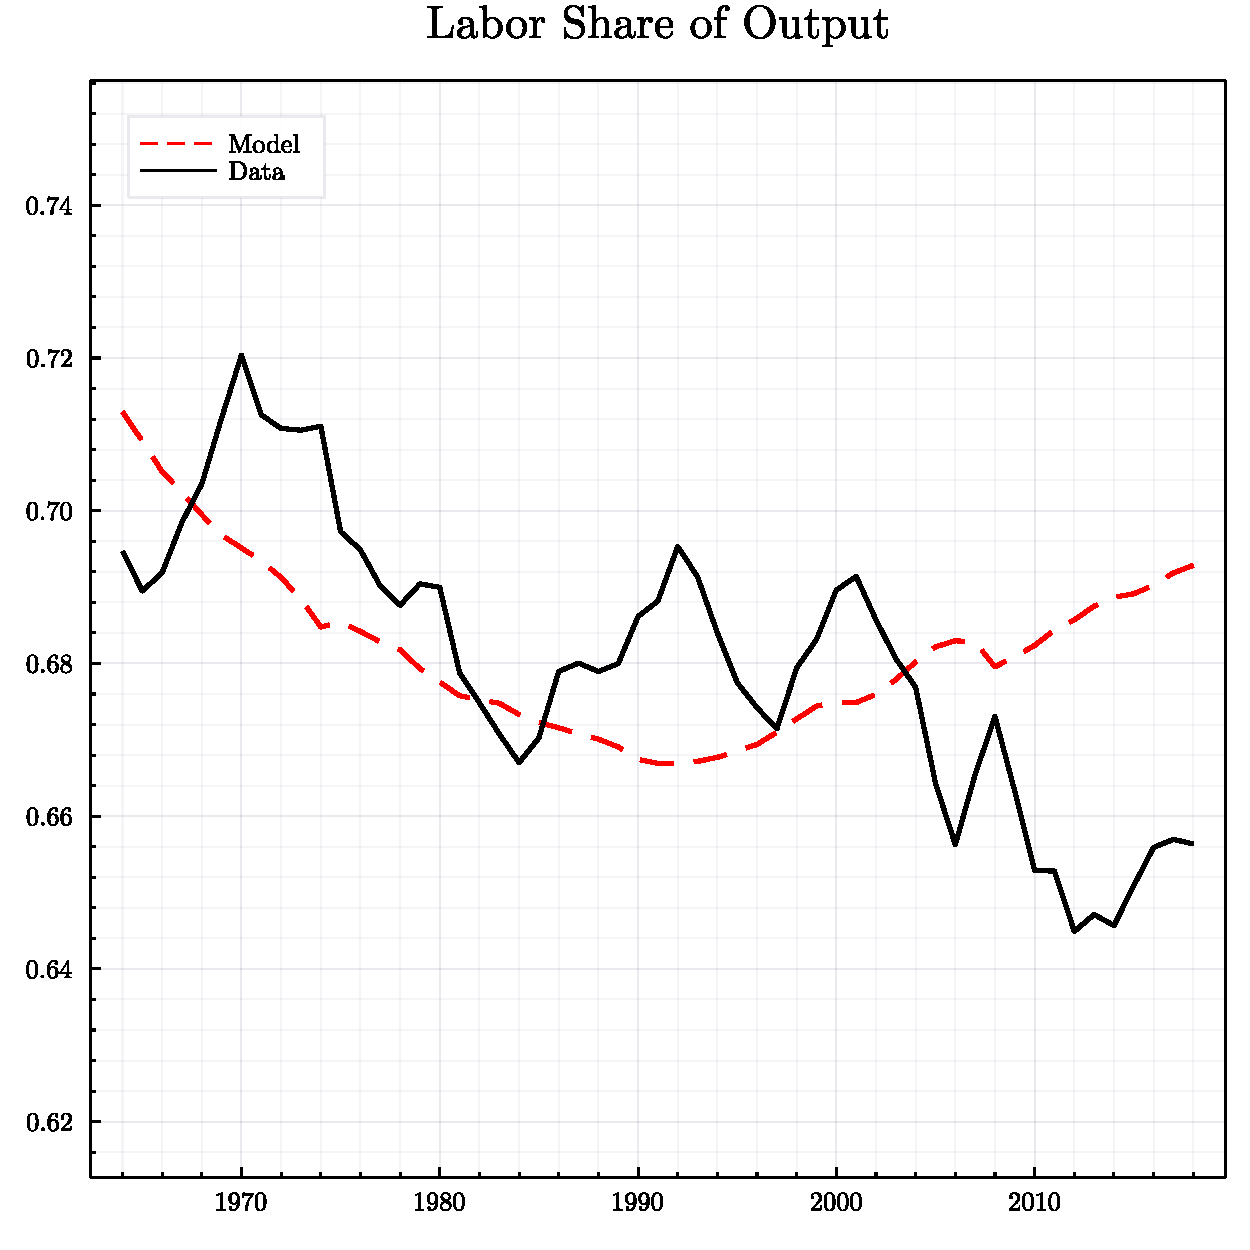
\includegraphics[width=0.3\textwidth]{../images/fig:updated_estimation_ls_doc.pdf}
 \hfill
 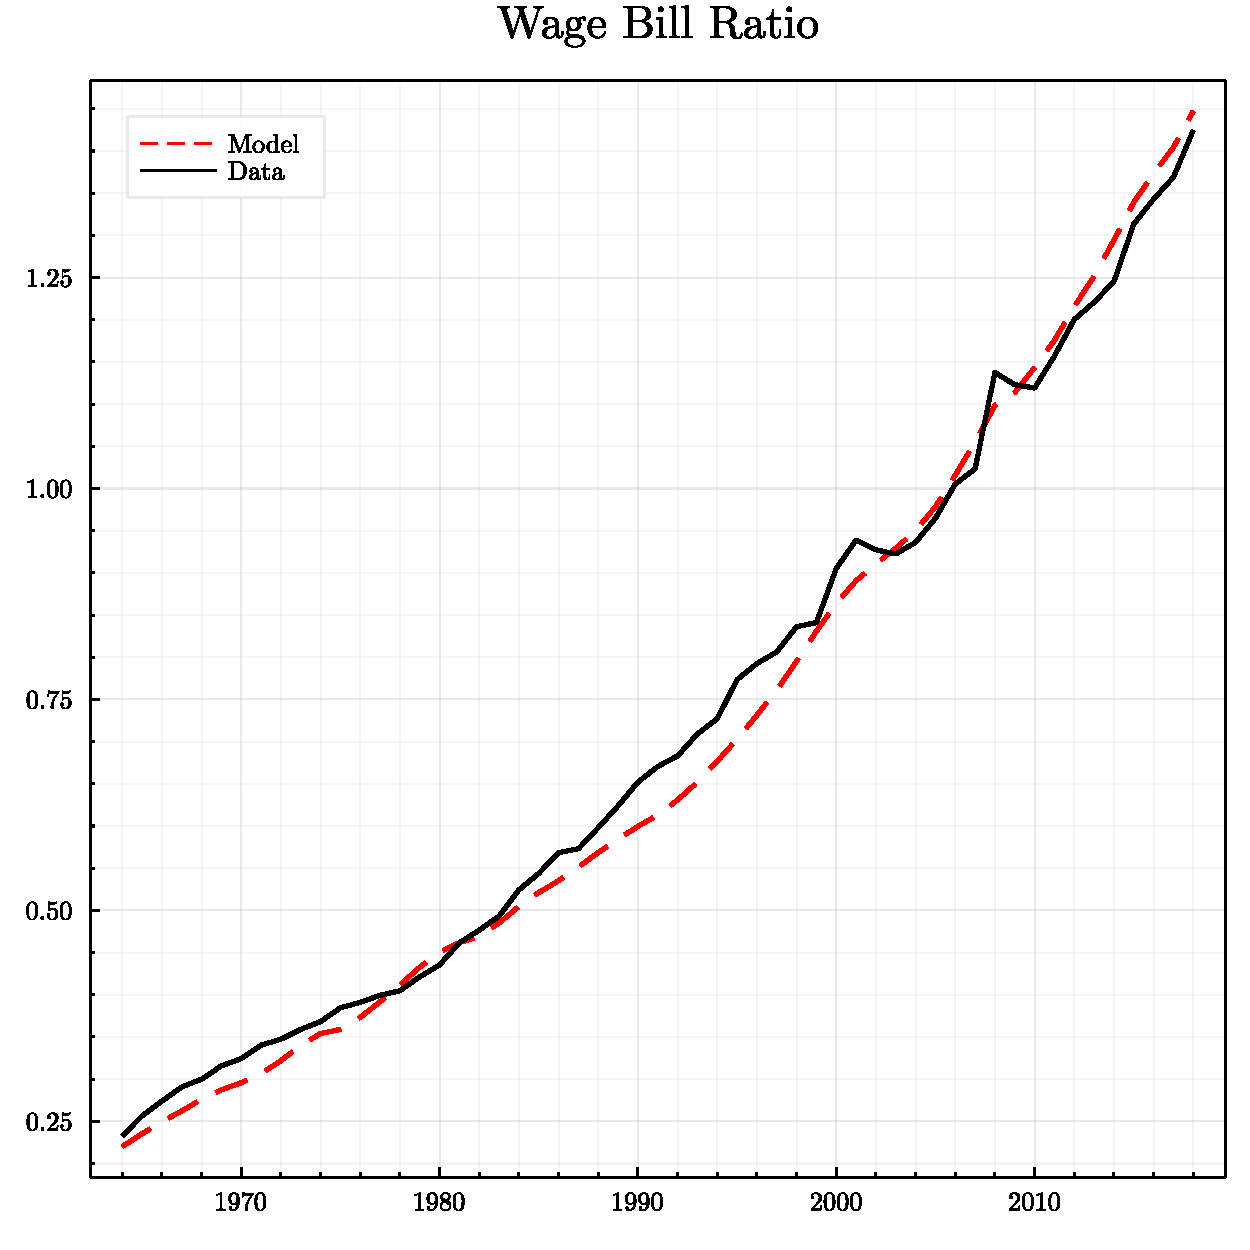
\includegraphics[width=0.3\textwidth]{../images/fig:updated_estimation_wbr_doc.pdf}
 \hfill
 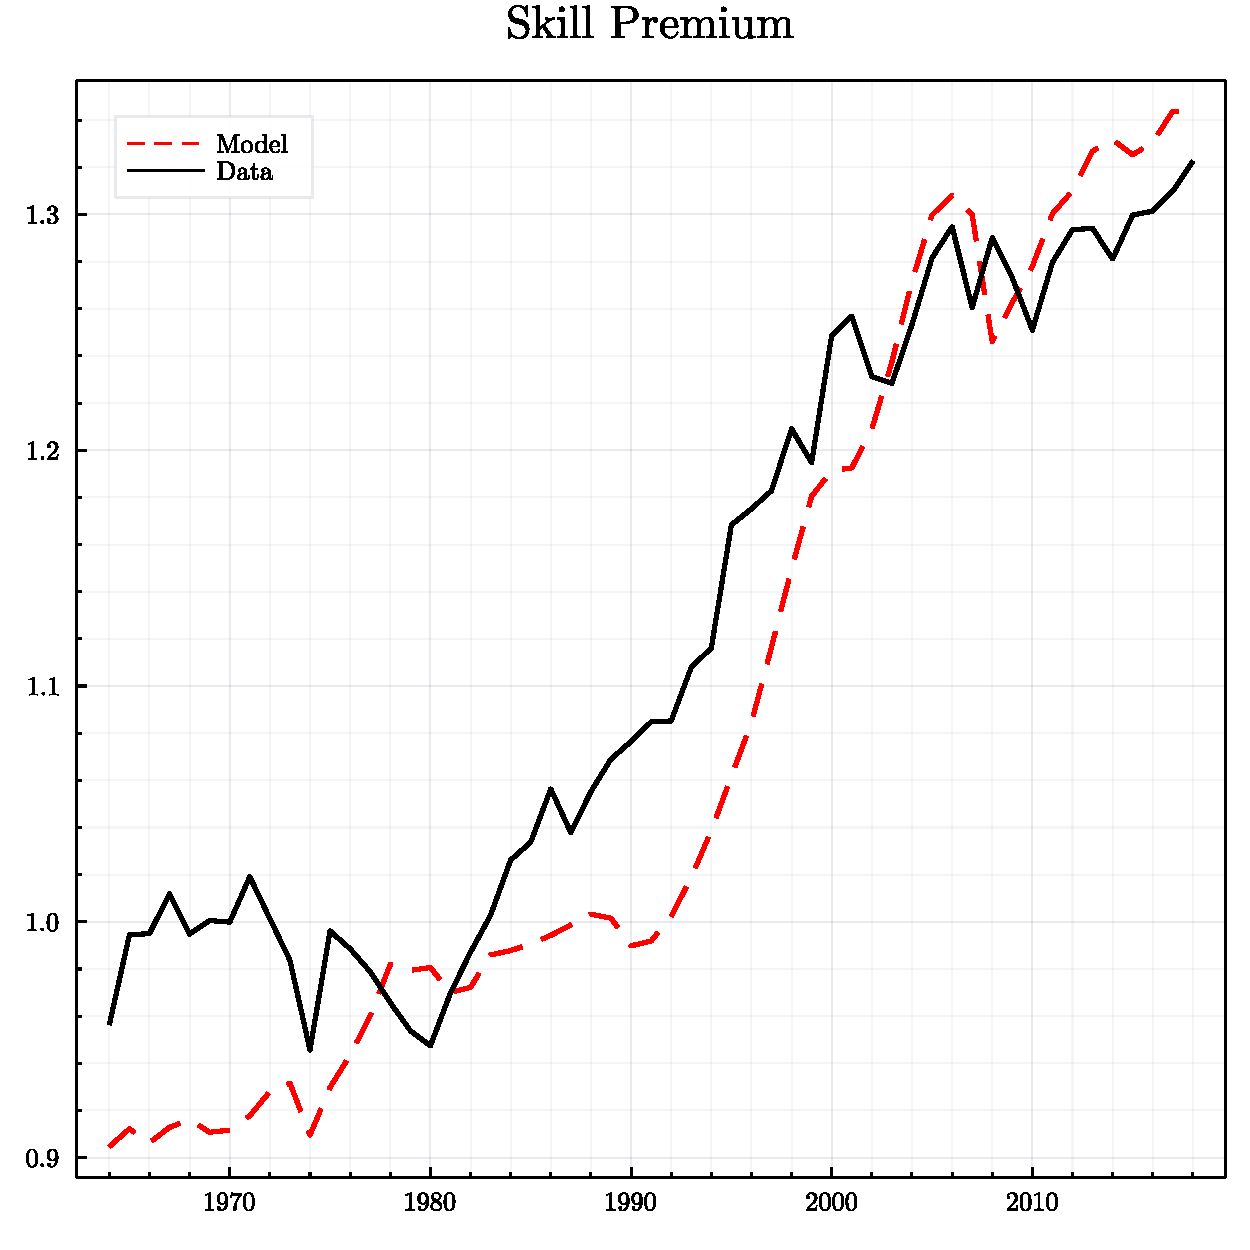
\includegraphics[width=0.3\textwidth]{../images/fig:updated_estimation_sp_doc.pdf}
 \caption{\label{fig:korv_estimation_extended} The model Fit for the $1963$ - $2018$ period with Updated Data.}
\end{figure}
\begin{figure}[H]
 \centering
 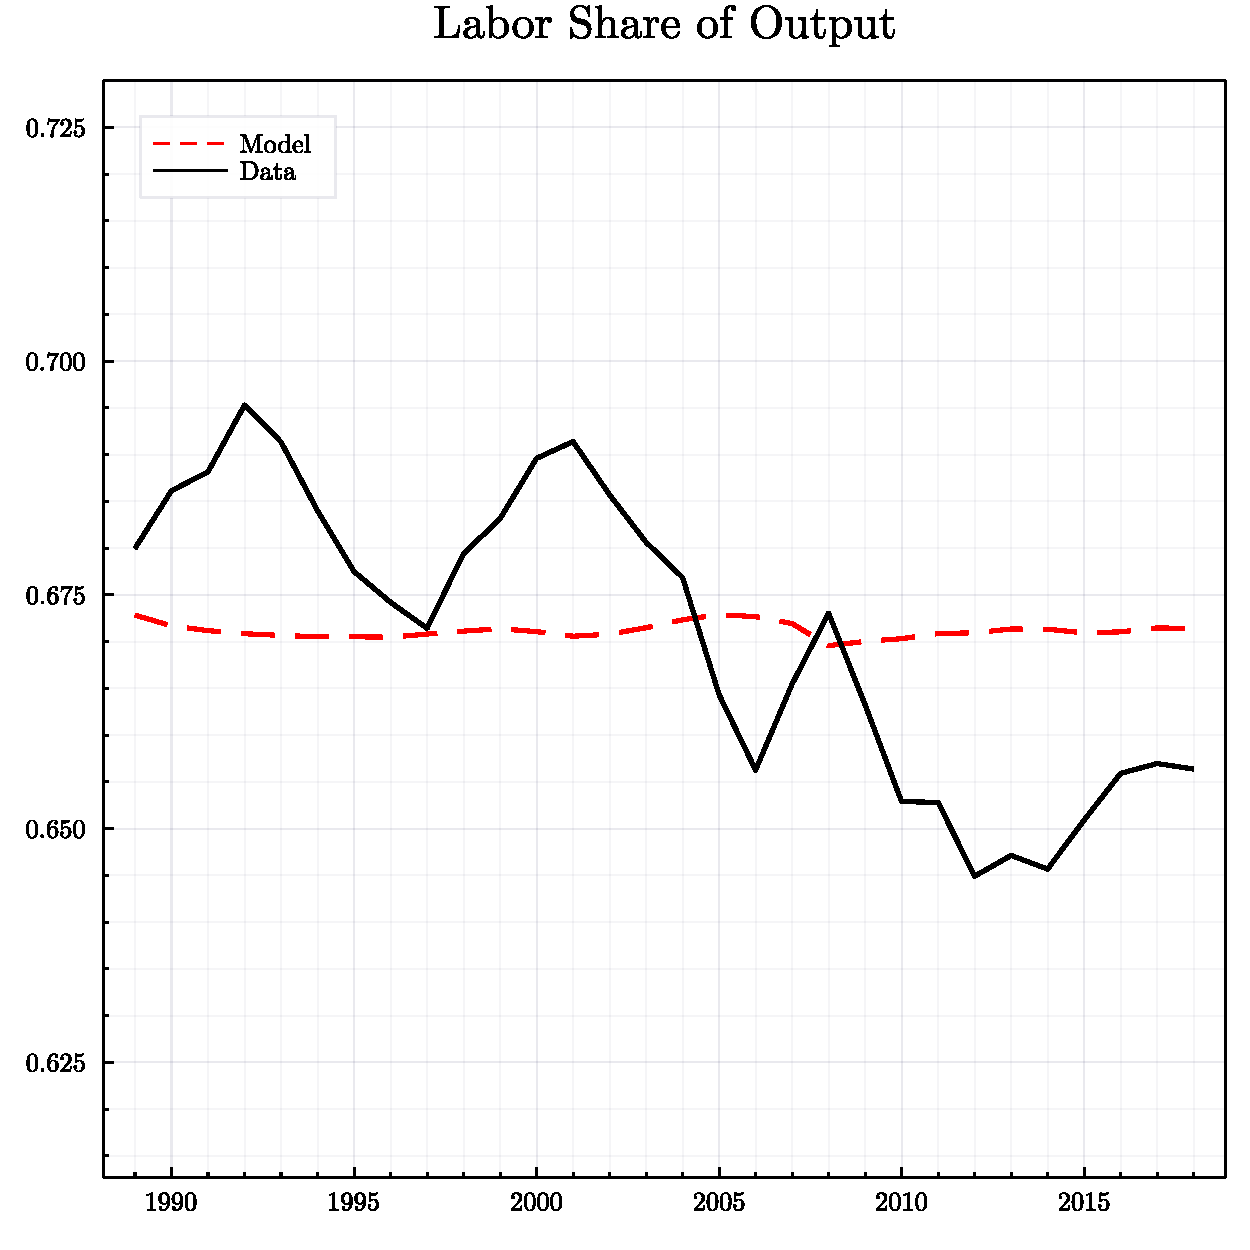
\includegraphics[width=0.3\textwidth]{../images/fig:updated_ind_estimation_ls_doc.pdf}
 \hfill
 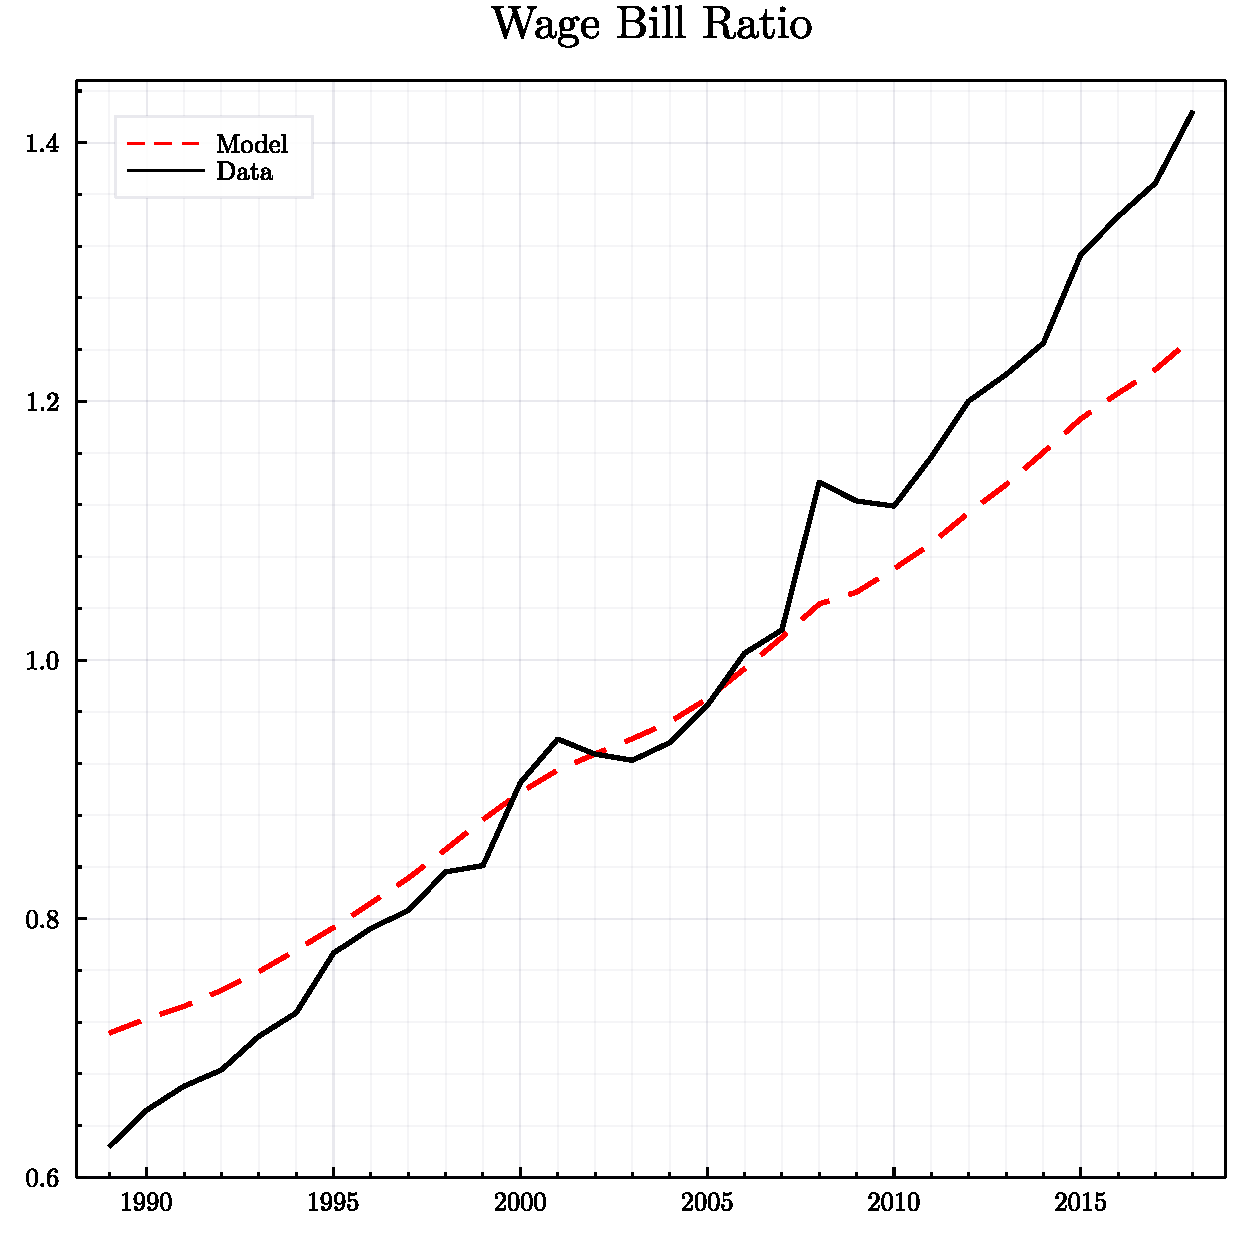
\includegraphics[width=0.3\textwidth]{../images/fig:updated_ind_estimation_wbr_doc.pdf}
 \hfill
 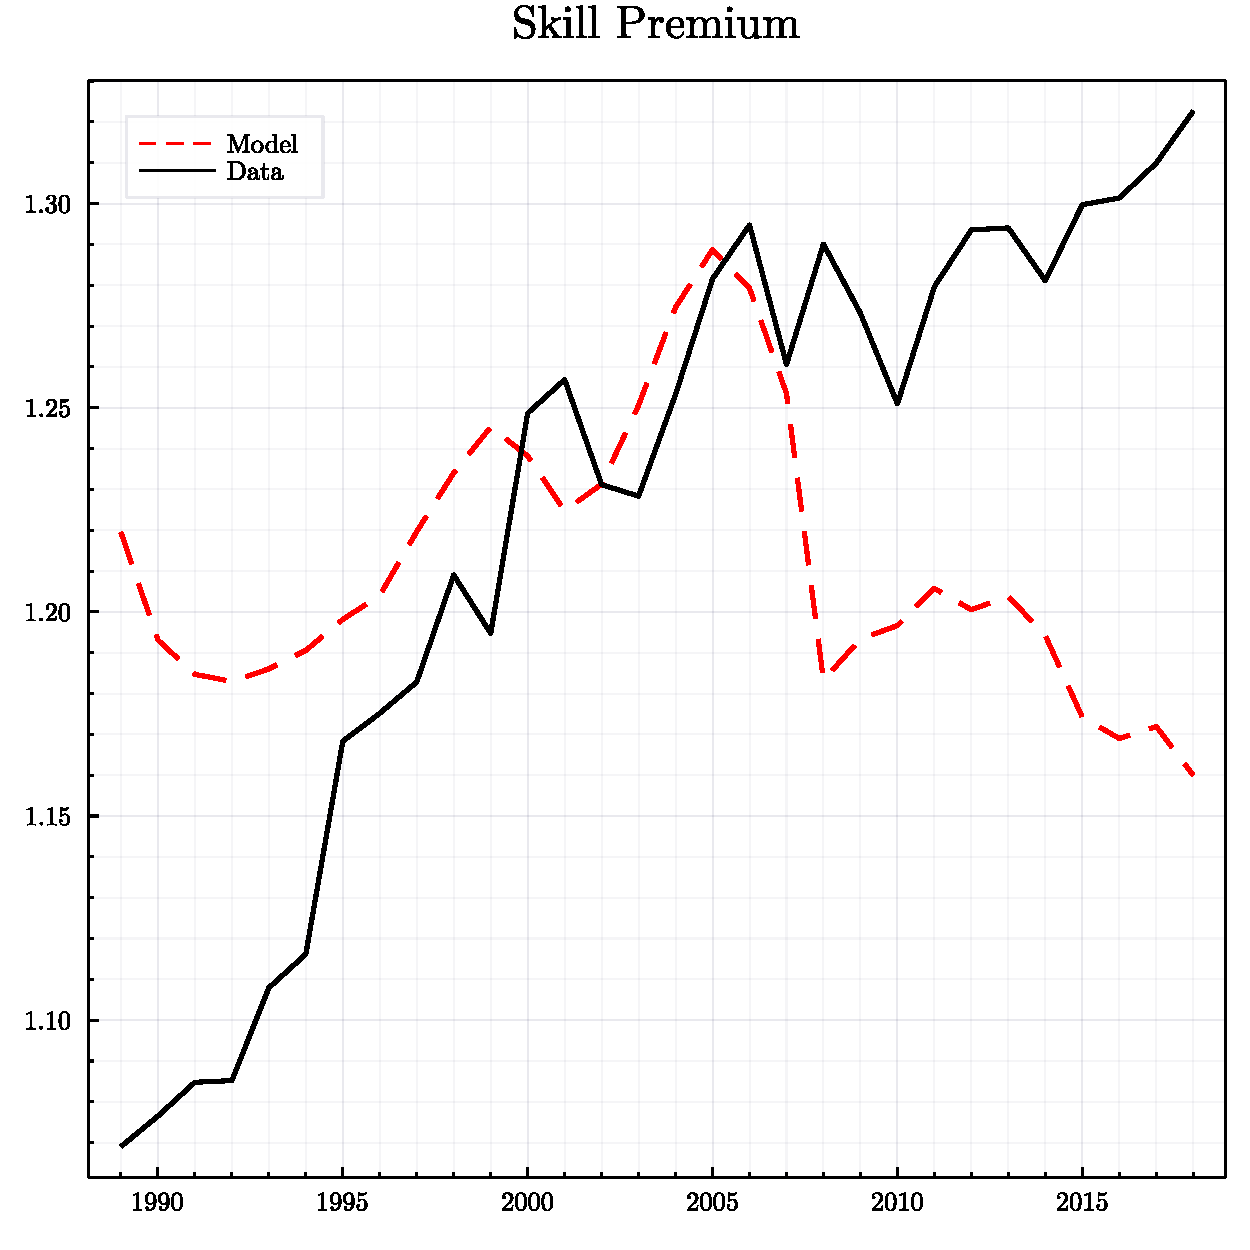
\includegraphics[width=0.3\textwidth]{../images/fig:updated_ind_estimation_sp_doc.pdf}
 \caption{\label{fig:korv_estimation_extended_industry} The model Fit for the $1988$ - $2018$ period with Updated Data.}
\end{figure}


As seen in table \ref{tab:estimation_korv} \textcolor{red}{Descirbe results}\dots


\subsection{Estimation by Industry}


\pagebreak{}

\bibliographystyle{chicago}
\bibliography{references}

\pagebreak{}

\appendix

\section{Ommited Derivations}\label{sec:derivations}
Outline:
\begin{itemize}
 \item FOC of Labor and Skill premium
 \item Log Linearization
 \item Write it as growth rates
\end{itemize}
To obtain a version of skill premium in terms of growth rates, start by writing a continuous time version of Equaiton~\eqref{eq:skill_premium_log_linear}:

\begin{equation}\label{eq:skill_premium_log_linear_continuous}
 \ln{\omega(t)} = \lambda \frac{\sigma-\rho}{\rho}\left(\frac{k_{e}(t)}{\psi^s(t) s(t) }\right)^\rho + (1-\sigma)\ln{\left(\frac{u(t)}{s(t)}\right)} + \sigma\ln{\left(\frac{\psi^s(t)}{\psi^u(t)}\right)}
\end{equation}
 
Start with the first term of the sum in the RHS:

\begin{align*}
 \frac{\partial}{\partial t}\left(\left(\frac{k_{e}(t)}{\psi^(t) s(t) }\right)^\rho\right) &= \rho\left( \frac{ k_e'(t)}{\psi^s(t) s(t)} - k_e(t) \frac{\psi'^s(t) s(t) + \psi^s(t) s'(t)}{(\psi^s(t) s(t))^2} \right)\left(\frac{k_{e}(t)}{\psi^s(t) s(t) }\right)^{\rho-1} \\
 &= \rho\left( \frac{ k_e'(t) k_e(t)}{k_e(t)(\psi^s(t) s(t)} - k_e(t) \frac{\psi'^s(t) s(t) + \psi^s(t) s'(t)}{(\psi^s(t) s(t))^2} \right)\left(\frac{k_{e}(t)}{\psi^s(t) s(t) }\right)^{\rho-1}\\
 &= \rho\left(\frac{k_e(t)}{\psi^s(t) s(t)}\right)^{\rho} \left( \frac{ k_e'(t) }{k_e(t)} - \frac{\psi'^s(t) s(t) + \psi^s(t) s'(t)}{\psi^s(t) s(t)} \right)\\
 &= \rho\left(\frac{k_e(t)}{\psi^s(t) s(t)}\right)^{\rho} \left( \frac{ k_e'(t) }{k_e(t)} - \frac{\psi'^s(t)}{\psi^s(t)} - \frac{ s'(t)}{ s(t)} \right)\\
 &= \rho\left(\frac{k_e(t)}{\psi^s(t) s(t)}\right)^{\rho}(g_{k_{e_{t}}} - g_{\psi^s_t} - g_{s_t})
\end{align*}

The next two terms in the sum are very similar, for the first term we have:

\begin{equation}
 \frac{\partial}{\partial t} \left( \ln{\left( \frac{\ell(t) }{s(t)} \right)} \right) = \frac{\partial}{\partial t} \left( \ln{\ell(t)} - \ln{(s(t)} \right) = \frac{\ell'(t)}{\ell(t)} - \frac{s'(t)}{s(t)} = g_{\ell_t} - g_{s_t}
\end{equation}
 
Differentiating the LHS we get:
$$\frac{\partial}{\partial t}\left(\ln{\omega(t)}\right) = \frac{\omega'(t)}{\omega(t)} = g_{\omega_t}$$


\section{Data Construction}\label{sec:data-construction}


\subsection{Capital Inputs and Labor Share}\label{subsec:capital-inputs-labor-share}
OUTLINE
\begin{itemize}
 \item Mention why are those delators used.
 \item How is the depreciation rate constructed?
\end{itemize}

% # After looking up the same for Structures and Intelectual Property I get:
% # * Stock of Capital:
% # - (FAAt301S) Table 3.1S. Current-Cost net Stock of Private Structures by Industry
% # - (FAAt301I) Table 3.1I. Current-Cost Net Stock of Intellectual Property Products by Industry
% # * Investment:
% # - (FAAt307S) Table 3.7S. Investment in Private Structures by Industry
% # - (FAAt307I) Table 3.7I. Investment in Private Intellectual Property Products by Industry
% # * Depreciation:
% # - (FAAt304S) Table 3.4S. Current-Cost Depreciation of Private Structures by Industry
% # - (FAAt304I) Table 3.4I. Current-Cost Depreciation of Private Intellectual Property Products by Industry

\subsection{Labor Inputs and Wage Rates}\label{subsec:labor-inputs-wage-rates}
I include all observations excluding agents: younger than $16$ or older than $70$, unpaid family workers, those working in the military, those who report working less than $40$ weeks a year and/or $35$ hours a week, individuals with allocated income, those with hourly wages below half of the minimum federal wage rate, those did not report their education level and self-employed workers.

For each person, I record their characteristics age, sex, and race. Their employment statistics: employment status (\texttt{empstat}), class of worker (\texttt{classwly}), weeks worked last year (\texttt{wkswork1} and \texttt{wkswork2}), usual hours worked per week last year (\texttt{uhrsworkly} and hours work last week \texttt{ahrsworkt}). Their income: total wage and salary income \texttt{incwage} and the CPS personal supplement weights: \texttt{asecwt}.

To homogenize the data I create the following groups based on individual characteristics, age is divided into 11 five-year groups: $16-20$, $21-25$, $26-30$, $31-35$,$36-40$,$41-45$,$46-50$ race is divided into white black and others. Sex is divided into, male and female and education is divided into four groups without high school, high school, some college and college graduates, and beyond. Then, each person is assigned to one of 264 groups created by age, race, sex, and skill (education).

For the period between $1963$ to $1975$ the variables weeks worked last year (\texttt{wkswork1}) and hours worked last year (\texttt{uhrsworkly}) are not recorded so I did the following substitution: For \texttt{wkswork1} we can use the variable \texttt{wkswork2} that consist of intervals of hours worked, and then perform the substitution with the average hours worked by individuals in the same group reporting the same value of \texttt{wkswork2} for the post $1975$ period. For \texttt{uhrsworkly} I used hours worked last week (\texttt{ahrsworkt}) as a proxy.

For every individual I create the following variables:
\begin{itemize}
\item $\ell_{i,t}$ the hours worked by individual $i$ in year $t$, is the product of hours worked per week times weeks worked that year.
\item $w_{i,t}$ the hourly wage of individual $i$ in year $t$, obtained by dividing yearly wage income by hours worked in year $t$.
\end{itemize}

Let $\mathcal{G}$ be the collection of all groups we can calculate the weight of each group as $\mu_{g,t} = \sum_{i\in g} \mu_{i,t}$ where $ \mu_{i,t}$ is the CPS weight of the individual. Average hours worked for each group $g\in\mathcal{G}$: 
\[
\ell_{g, t-1} = \frac{\sum_{i\in g}\ell_{i,t-1} \mu_{i,t}}{\mu_{g, t}}
\]
and wages:
\[
w_{g, t-1} = \frac{\sum_{i\in g}w_{i,t-1} \mu_{i,t}}{\mu_{g, t}}
\]
Finally to obtain skilled and unskilled series labor input and wage series I partitioned the set $\mathcal{G}$ in two subsets $(\mathcal{S}, \mathcal{U})$ based on education (college graduates and non-college graduates). Let $\{H, L\}$ indicate the group type, then the total labor input is:
\[
 L^U_{t-1} = \sum_{g \in\mathcal{U}} \ell_{g, t-1} \mu_{g,t} w_{g,80}
\]
\[
 L^S_{t-1} = \sum_{g \in\mathcal{S}} \ell_{g, t-1} \mu_{g,t} w_{g,80}
\]
$w_{g,80}$ is the wage of the group in 1980 and is used as a scaling factor. Then wages for each skill level are obtained as:
\[
W^U_{t-1} = \frac{\sum_{g \in \mathcal{U}} w_{g, t-1} \ell_{g, t-1} \mu_{g,t}}{L^U_{t-1}}
\]
\[
W^S_{t-1} = \frac{\sum_{g \in \mathcal{S}} w_{g, t-1} \ell_{g, t-1} \mu_{g,t}}{L^S_{t-1}}
\]

\section{Industry Specific Trends}\label{sec:industry-specific-trends}

\end{document}